\documentclass[openany]{book}

\usepackage[margin=1in]{geometry}
\usepackage{amsmath,amsfonts,amsthm, amssymb}
\usepackage{yhmath}
\usepackage{mathrsfs}
\usepackage{mathtools}
\usepackage{xcolor}
\usepackage{graphicx}
\usepackage{comment}
\usepackage{tikz-cd}
\usepackage{quiver}
\renewcommand{\familydefault}{ppl}
\newcommand{\tr}{\text{tr}}
\newcommand{\R}{\mathbb{R}}
\newcommand{\E}{\mathbb{E}}
\newcommand{\Z}{\mathbb{Z}}
\newcommand{\C}{\mathbb{C}}
\newcommand{\F}{\mathbb{F}}
\newcommand{\la}{\langle}
\newcommand{\ra}{\rangle}
\newcommand{\aut}{\text{Aut}}
\newcommand{\colim}{\text{colim}}
\DeclareMathOperator{\im}{im}
\let\oldemptyset\emptyset
\let\emptyset\varnothing
\newcommand{\tor}{\text{Tor}}
\newcommand{\id}{\text{id}}
\newcommand{\ext}{\text{Ext}}
\newcommand{\ptop}{\text{PTop}}
\newcommand{\pt}{\text{pt}}
\newcommand{\ach}{\text{Ach}}
\newcommand{\Q}{\mathbb{Q}}
\newcommand{\gal}{\text{Gal}}


\usepackage{thmtools,thm-restate}

% Fixing mdframed skip below
% See https://tex.stackexchange.com/a/292090/143086
\usepackage[framemethod=TikZ]{mdframed}
\usepackage{xpatch}
\makeatletter
\xpatchcmd{\endmdframed}
	{\aftergroup\endmdf@trivlist\color@endgroup}
	{\endmdf@trivlist\color@endgroup\@doendpe}
	{}{}
\makeatother

\definecolor{huilightpink}{HTML}{fff2fe}
\definecolor{huidarkpink}{HTML}{d955b7}
\declaretheoremstyle[
	mdframed={
		backgroundcolor=huilightpink,
		linecolor=huidarkpink,
		rightline=false,
		topline=false,
		bottomline=false,
		linewidth=2pt,
		innertopmargin=5pt,
		innerbottommargin=8pt,
		innerleftmargin=8pt,
		leftmargin=-2pt,
		skipbelow=2pt,
		nobreak
	},
	headfont=\normalfont\bfseries\color{huidarkpink}
]{huipinkbox}
\declaretheorem[style=huipinkbox,name=Theorem,within=chapter]{thm}
\declaretheorem[style=huipinkbox,name=Theorem,sibling=thm]{theorem}




\begin{comment}
\definecolor{huilightyellow}{HTML}{fff5d6}
\definecolor{huidarkyellow}{HTML}{fcad03}
\declaretheoremstyle[
	mdframed={
		backgroundcolor=huilightyellow,
		linecolor=huidarkyellow,
		rightline=false,
		topline=false,
		bottomline=false,
		linewidth=2pt,
		innertopmargin=5pt,
		innerbottommargin=8pt,
		innerleftmargin=8pt,
		leftmargin=-2pt,
		skipbelow=2pt,
		nobreak
	},
	headfont=\normalfont\bfseries\color{huidarkyellow}
]{huiyellowbox}
\declaretheorem[style=huiyellowbox,name=Proposition,within=chapter]{prop}
\end{comment}



\definecolor{huilightpurple}{HTML}{faf2ff}
\definecolor{huidarkpurple}{HTML}{912ed9}
\declaretheoremstyle[
	mdframed={
		backgroundcolor=huilightpurple,
		linecolor=huidarkpurple,
		rightline=false,
		topline=false,
		bottomline=false,
		linewidth=2pt,
		innertopmargin=5pt,
		innerbottommargin=8pt,
		innerleftmargin=8pt,
		leftmargin=-2pt,
		skipbelow=2pt,
		nobreak
	},
	headfont=\normalfont\bfseries\color{huidarkpurple}
]{huipurplebox}
\declaretheorem[style=huipurplebox,name=Proposition,within=chapter]{prop}



% \definecolor{huilightpurple}{HTML}{faf2ff}
% \definecolor{huidarkpurple}{HTML}{912ed9}
% \declaretheoremstyle[
% 	mdframed={
% 		backgroundcolor=huilightpurple,
% 		linecolor=huidarkpurple,
% 		rightline=false,
% 		topline=false,
% 		bottomline=false,
% 		linewidth=2pt,
% 		innertopmargin=5pt,
% 		innerbottommargin=8pt,
% 		innerleftmargin=8pt,
% 		leftmargin=-2pt,
% 		skipbelow=2pt,
% 		nobreak
% 	},
% 	headfont=\normalfont\bfseries\color{huidarkpurple}
% ]{huipurplebox}
\declaretheorem[style=huipurplebox,name=Lemma,within=chapter]{lem}


\definecolor{lightpink}{HTML}{f0f6fc}
\definecolor{darkpink}{HTML}{2c72b8}
\declaretheoremstyle[
	mdframed={
		backgroundcolor=lightpink,
		linecolor=darkpink,
		rightline=false,
		topline=false,
		bottomline=false,
		linewidth=2pt,
		innertopmargin=5pt,
		innerbottommargin=8pt,
		innerleftmargin=8pt,
		leftmargin=-2pt,
		skipbelow=2pt,
		nobreak
	},
	headfont=\normalfont\bfseries\color{darkpink}
]{pinkbox}
\declaretheorem[style=pinkbox,name=Definition,within=chapter]{defn}


\definecolor{huilightblue}{HTML}{edf9ff}
\definecolor{huidarkblue}{HTML}{4b79db}
\declaretheoremstyle[
	mdframed={
		backgroundcolor=huilightblue,
		linecolor=huidarkblue,
		rightline=false,
		topline=false,
		bottomline=false,
		linewidth=2pt,
		innertopmargin=5pt,
		innerbottommargin=8pt,
		innerleftmargin=8pt,
		leftmargin=-2pt,
		skipbelow=2pt,
		nobreak
	},
	headfont=\normalfont\bfseries\color{huidarkblue}
]{huiblueblox}
\declaretheorem[style=huiblueblox,name=Example,within=chapter]{example}



% \definecolor{huilightblue}{HTML}{edf9ff}
% \definecolor{huidarkblue}{HTML}{4b79db}
% \declaretheoremstyle[
% 	mdframed={
% 		backgroundcolor=huilightblue,
% 		linecolor=huidarkblue,
% 		rightline=false,
% 		topline=false,
% 		bottomline=false,
% 		linewidth=2pt,
% 		innertopmargin=5pt,
% 		innerbottommargin=8pt,
% 		innerleftmargin=8pt,
% 		leftmargin=-2pt,
% 		skipbelow=2pt,
% 		nobreak
% 	},
% 	headfont=\normalfont\bfseries\color{huidarkblue}
% ]{huiblueblox}
% \declaretheorem[style=huiblueblox,name=Example,within=chapter]{example}

% \declaretheoremstyle[
% 	mdframed={
% 		backgroundcolor=huilightblue,
% 		linecolor=huidarkblue,
% 		rightline=false,
% 		topline=false,
% 		bottomline=false,
% 		linewidth=2pt,
% 		innertopmargin=5pt,
% 		innerbottommargin=8pt,
% 		innerleftmargin=8pt,
% 		leftmargin=-2pt,
% 		skipbelow=2pt,
% 		nobreak
% 	},
% 	headfont=\normalfont\bfseries\color{huidarkblue}
% ]{huiblueblox}
\declaretheorem[style=huiblueblox,name=Problem,within=chapter]{prob}



% \declaretheoremstyle[
% 	mdframed={
% 		backgroundcolor=huilightblue,
% 		linecolor=huidarkblue,
% 		rightline=false,
% 		topline=false,
% 		bottomline=false,
% 		linewidth=2pt,
% 		innertopmargin=5pt,
% 		innerbottommargin=8pt,
% 		innerleftmargin=8pt,
% 		leftmargin=-2pt,
% 		skipbelow=2pt,
% 		nobreak
% 	},
% 	headfont=\normalfont\bfseries\color{huidarkblue}
% ]{huiblueblox}
\declaretheorem[style=huiblueblox,name=Exercise,within=chapter]{exer}
\declaretheorem[style=huipinkbox, name=Corollary, within=chapter]{cor}





















\newcommand{\nirwarnsymbol}{%
	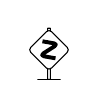
\begin{tikzpicture}[baseline=(x.base)]
		\draw[rounded corners=.01em] (-.05em,-1.07em)rectangle(.05em,.78em);
		\draw[fill=white,rounded corners=1.3] (0,.75em)--(.75em,0)--(0,-.75em)--(-.75em,0)--cycle;
		\draw[line width=0.2mm, line cap=round](-.4em,-1.07em)--(.4em,-1.07em);
		\node(x) at (0,0em) {};
		% Thank you https://tex.stackexchange.com/a/262510
		\draw[
			line cap=but,
			line join=round,
			x=.5em,
			line width=0.5mm,
			y=1*(height("Z")-\pgflinewidth)*(1-sin(10)),
			rotate=-10,
			rounded corners=1.5pt,
		](-0.57, 0.57) -- (0.57, 0.57) -- (-0.57, -0.57) -- (0.57, -0.57);
	\end{tikzpicture}%
}

%%%%%%%%%%%%%%%%%%%%%%%%%%%%%%%%%%%%%%%%%%%% MARGINS
\usepackage{marginnote}
% Thank you https://tex.stackexchange.com/a/472882
% Makes marginnotes always appear on the left, apparently
%
\makeatletter
\long\def\@mn@@@marginnote[#1]#2[#3]{%
	\begingroup
		\ifmmode\mn@strut\let\@tempa\mn@vadjust\else
			\if@inlabel\leavevmode\fi
			\ifhmode\mn@strut\let\@tempa\mn@vadjust\else\let\@tempa\mn@vlap\fi
		\fi
		\@tempa{%
			\vbox to\z@{%
				\vss
				\@mn@margintest
				\if@reversemargin\if@tempswa
						\@tempswafalse
					\else
						\@tempswatrue
				\fi\fi

					\llap{%
						\vbox to\z@{\kern\marginnotevadjust\kern #3
							\vbox to\z@{%
								\hsize\marginparwidth
								\linewidth\hsize
								\kern-\parskip
								%\mn@parboxrestore
								\marginfont\raggedleftmarginnote\strut\hspace{\z@}%
								\ignorespaces#1\endgraf
								\vss
							}%
							\vss
						}%
						\if@mn@verbose
							\PackageInfo{marginnote}{xpos seems to be \@mn@currxpos}%
						\fi
						\begingroup
							\ifx\@mn@currxpos\relax\else\ifx\@mn@currpos\@empty\else
									\kern\@mn@currxpos
							\fi\fi
							\ifx\@mn@currpage\relax
								\let\@mn@currpage\@ne
							\fi
							\if@twoside\ifodd\@mn@currpage\relax
									\kern-\oddsidemargin
								\else
									\kern-\evensidemargin
								\fi
							\else
								\kern-\oddsidemargin
							\fi
							\kern-1in
						\endgroup
						\kern\marginparsep
					}%
			}%
		}%
	\endgroup
}
\makeatother
%
% Mostly for todonotes
\renewcommand{\marginpar}{\marginnote}
%%%%%%%%%%%%%%%%%%%%%%%%%%%%%%%%%%%%%%%%%%%% /MARGINS

\definecolor{nirlightred}{RGB}{250, 220, 220}
\definecolor{nirdarkred}{HTML}{f40000}
\declaretheoremstyle[
	mdframed={
		backgroundcolor=nirlightred,
		linecolor=nirdarkred,
		rightline=false,
		topline=false,
		bottomline=false,
		linewidth=2pt,
		innertopmargin=5pt,
		innerbottommargin=8pt,
		innerleftmargin=8pt,
		leftmargin=-2pt,
		skipbelow=2pt,
		nobreak
	},
	headfont=\normalfont\bfseries\color{nirdarkred}
]{nirredbox}

% \makeatletter
% \declaretheorem[
% 	style=nirredbox,
% 	name=Warning,
% 	sibling=thm,
% 	% without \leavevmode, the first item in a list gets misformatted
% 	postheadhook={\leavevmode\marginnote{\nirwarnsymbol}[-3pt]%
% 	\ifthmt@thisistheone% restatable makes alignment weird
% 		\hspace{-2.2pt}%
% 	\fi}
% ]{warn}
% \makeatother

\newcommand{\nirideasymbol}{%
	
\begin{tikzpicture}[baseline=(x.base)]
		\draw[rounded corners=.01em] (-.05em,-1.07em)rectangle(.05em,.78em);
		\draw[fill=white,rounded corners=1.3] (0,.75em)--(.75em,0)--(0,-.75em)--(-.75em,0)--cycle;
		\draw[line width=0.2mm, line cap=round](-.4em,-1.07em)--(.4em,-1.07em);
		\node(x) at (0,0em) {};
		\node at (0,0em) {{\textbf{!}}};
	\end{tikzpicture}%
}
\renewcommand{\nirwarnsymbol}{%
	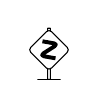
\begin{tikzpicture}[baseline=(x.base)]
		\draw[rounded corners=.01em] (-.05em,-1.07em)rectangle(.05em,.78em);
		\draw[fill=white,rounded corners=1.3] (0,.75em)--(.75em,0)--(0,-.75em)--(-.75em,0)--cycle;
		\draw[line width=0.2mm, line cap=round](-.4em,-1.07em)--(.4em,-1.07em);
		\node(x) at (0,0em) {};
		% Thank you https://tex.stackexchange.com/a/262510
		\draw[
			line cap=but,
			line join=round,
			x=.5em,
			line width=0.5mm,
			y=1*(height("Z")-\pgflinewidth)*(1-sin(10)),
			rotate=-10,
			rounded corners=1.5pt,
		](-0.57, 0.57) -- (0.57, 0.57) -- (-0.57, -0.57) -- (0.57, -0.57);
	\end{tikzpicture}%
}
\makeatletter
\declaretheorem[
	style=nirredbox,
	name=Idea,
	sibling=thm,
	% without \leavevmode, the first item in a list gets misformatted
	postheadhook={\leavevmode\marginnote{\nirideasymbol}[-3pt]%
	\ifthmt@thisistheone% restatable makes alignment weird
		\hspace{-2.2pt}%
	\fi}
]{idea}

\declaretheorem[
	style=nirredbox,
	name=Warning,
	sibling=thm,
	% without \leavevmode, the first item in a list gets misformatted
	postheadhook={\leavevmode\marginnote{\nirwarnsymbol}[-3pt]%
	\ifthmt@thisistheone% restatable makes alignment weird
		\hspace{-2.2pt}%
	\fi}
]{warn}
\makeatother

\title{Aluffi Problems}

\date{\today}
\author{Hui Sun}


\begin{document}

\maketitle

\tableofcontents
\newpage

\chapter{Category Theory}

\chapter{Groups I}

\begin{prob}[1.8]
    Let \( G \) be a finite abelian group with exactly one element \( f \) of order 2. Prove that \(\prod_{g \in G} g = f\).
\end{prob}
\begin{proof}
    It suffices to see that $\prod_gg^2=e$, which is true by every element has an inverse.
\end{proof}










\begin{prob}[1.13]
    Give an example showing that \( |gh| \) is not necessarily equal to \( \text{lcm}(|g|, |h|) \), even if \( g \) and \( h \) commute.
\end{prob}
\begin{proof}
    Let $g=h=1\in\Z/2\Z$.
\end{proof}

\begin{prob}[1.14]
    If \( g \) and \( h \) commute and \( \text{gcd}(|g|, |h|) = 1 \), then \( |gh| = |g||h| \). (Hint: Let \( N = |gh| \); then \( g^N = (h^{-1})^N \). What can you say about this element?)
\end{prob}
\begin{proof}
    We know that $g^N = (h^{-1})^N=e$.
\end{proof}

\begin{prob}[6.7]
    If $\mathrm{Aut}(G)$ is cyclic, then $G$ is abelian.
\end{prob}
\begin{proof}
    This implies $\text{Inn}(G)$ is cyclic, which is iff $\text{Inn}(G)$ is trivial, iff $G$ is abelian.
\end{proof}






\begin{prob}[6.9]
    Prove that every finitely generated subgroup of $\mathbb{Q}$ is cyclic. Prove that $\mathbb{Q}$ is not finitely generated.
\end{prob}
\begin{proof}
    Suppose we just have $H=\left\la\frac{p_1}{q_1}, \frac{p_2}{q_2}\right\ra$, find $\text{lcm}(q_1,q_2)=q$, then 
    \begin{equation*}
        H=\left\la\frac{a_1}{q},\frac{a_2}{q}\right\ra
    \end{equation*}
    find $\gcd(a_1,a_2)=p$, we claim that 
    \begin{equation*}
        H=\left\la\frac{p}{q}\right\ra
    \end{equation*}
    If $\Q$ were to be finitely generated, then it is cyclic, $\Q=\la\frac{p}{q}\ra$, then try $(p+1)/q$.
\end{proof}

\begin{prob}[8.1]
    If a group \( H \) may be realized as a subgroup of two groups \( G_1 \) and \( G_2 \) and if  
    \[
    \frac{G_1}{H} \cong \frac{G_2}{H},
    \]
    does it follow that \( G_1 \cong G_2 \)? Give a counterexample.
\end{prob}
\begin{proof}
    Let $G_1=S_3, G_2=\Z/6\Z$, and $H=\Z/3\Z$.
\end{proof}

\begin{prob}[8.2]
    Suppose \( G \) is a group and \( H \subseteq G \) is a subgroup of index 2, that is, such that there are precisely two cosets of \( H \) in \( G \). Prove that \( H \) is normal in \( G \).
\end{prob}
\begin{proof}
    For any $g\not\in H$, we have 
    \begin{equation*}
        G=H\sqcup gH=H\sqcup Hg
    \end{equation*}
    Thus $gH=Hg$.
\end{proof}


\begin{prob}[8.13]
    Let \( G \) be a finite group, and assume \(|G|\) is odd. Prove that every element of \( G \) is a square.
\end{prob}
\begin{proof}
    Consider the set function $\varphi:g\mapsto g^2$, this function is injective hence surjective.
\end{proof}


\begin{prob}[8.18]
    Let \( G \) be an abelian group of order \( 2n \), where \( n \) is odd. Prove that \( G \) has exactly one element of order 2. (It has at least one, for example by Exercise [8.17]. Use Lagrange's theorem to establish that it cannot have more than one.) Does the same conclusion hold if \( G \) is not necessarily commutative?
\end{prob}
\begin{proof}
    There exists one element $g$ of order $2$, then take its quotient $G/\la g\ra$. 
\end{proof}

\begin{prob}[9.11]
    Let $G$ be a finite group, and $H$ be subgroup of index $p$, where $p$ is the smallest prime dividing $|G|$, then $H$ is normal in $G$.
\end{prob}
\begin{proof}
    (I will abuse the notatoin $\left|\frac{G}{H}\right|=[G:H]$).
    Let $G$ act on the cosets $G/H$ by left multiplication, this action $\sigma: G\to\text{Aut}(G/H)$ is not trivial, hence 
    \begin{equation*}
        \left|\frac{G}{\ker(\sigma)}\right|\text{ divides } p!
    \end{equation*}
    Moreover, we notice that $\ker(\sigma)\subset H$, hence $p$ divides $\left|\frac{G}{\ker(\sigma)}\right|$. Now we recall that $p$ is the smallest prime dividing $|G|$, we must have $\left|\frac{G}{\ker(\sigma)}\right|=p$, hence $H=\ker(\sigma)$.
\end{proof}






















\begin{prop}[1.12]
    There exists elements $g,h\in G$, such that $|g|,|h|<\infty$, but $|gh|=\infty$.
    \[
    g = \begin{pmatrix}
    0 & -1 \\
    1 & 0
    \end{pmatrix}, \quad h = \begin{pmatrix}
    0 & 1 \\
    -1 & -1
    \end{pmatrix}.
    \]
\end{prop}



\begin{prop}[1.15]
    Let \( G \) be a commutative group, and let \( g \in G \) be an element of maximal finite order, that is, such that if \( h \in G \) has finite order, then \( |h| \leq |g| \). Then, if \( h \) has finite order in \( G \), then \( |h| \) divides \( |g| \).
\end{prop}


\begin{prop}
    When $n$ is odd, the center of $D_{2n}$ is trivial, when $n$ is even, the center consists of $\{e, r^\frac{n}{2}\}$.
    \begin{equation*}
        r^\frac{n}{2}s=sr^{-\frac{n}{2}}=sr^\frac{n}{2}
    \end{equation*}
\end{prop}


\begin{prop}[4.8]
    The map $g\mapsto \left(r_g: a\mapsto gag^{-1}\right)$ defines a homomorphism from $G\to \text{Aut}(G)$.
\end{prop}


\begin{prop}[4.9]
    Let $m,n$ be positive integers such that $\gcd(m,n)=1$, then 
    \begin{equation*}
        \frac{\Z}{mn\Z}\cong\frac{\Z}{m\Z}\times\frac{\Z}{n\Z}
    \end{equation*}
\end{prop}


\begin{prop}[4.14]
    The order of the group of automorphisms of $\Z/n\Z$ is the the number of generators of $\Z/\Z$, i.e., 
    \begin{equation*}
        \left|\text{Aut}(\Z/n\Z)\right|=\left|(\Z/n\Z)^\times\right|
    \end{equation*}
\end{prop}

\begin{prop}[4.15]
    Let $p$ be a prime, then 
    \begin{equation*}
        \text{Aut}(\Z/p\Z)\cong\frac{\Z}{(p-1)\Z}
    \end{equation*}
\end{prop}

\begin{prop}[6.3]
    Every matrix in $\mathrm{SU}(2)$ may be written in the form
    \[
    \begin{pmatrix}
    a + bi & c + di \\
    -c + di & a - bi
    \end{pmatrix}=\begin{pmatrix}
        \gamma&\omega\\
        -\bar{\omega}&\bar{\gamma}
    \end{pmatrix},
    \]
    where $a, b, c, d \in \mathbb{R}$ and $a^2 + b^2 + c^2 + d^2 = 1$.
\end{prop}


\begin{prop}[6.10]
    The set of \( 2 \times 2 \) matrices with integer entries and determinant 1 is denoted \(\text{SL}_2(\mathbb{Z})\):

\[
\text{SL}_2(\mathbb{Z}) = \left\{ 
\begin{pmatrix}
a & b \\
c & d
\end{pmatrix} 
\quad \text{such that } a, b, c, d \in \mathbb{Z}, \, ad - bc = 1 \right\}.
\]

Note that \(\text{SL}_2(\mathbb{Z})\) is generated by the matrices

\[
s = 
\begin{pmatrix}
0 & -1 \\
1 & 0
\end{pmatrix} \quad \text{and } \, t = 
\begin{pmatrix}
1 & 1 \\
0 & 1
\end{pmatrix}.
\]

\end{prop}

\begin{prop}[7.7]
    Let $G$ be a group and $n$ a positive integer, let $H\subset G$ be the subgroup generated by all elements of order $n$ in $G$, then $H$ is normal.
\end{prop}

\begin{prop}[7.14]
    $\text{Inn}(G)$ is a normal subgroup of $\text{Aut}(G)$.
\end{prop}

\begin{prop}[8.4]
    The dihedral group $D_{2n}$ can also be represented as 
    \begin{equation*}
        \la a,b: a^2=b^2=(ab)^n=e\ra
    \end{equation*}
    ($a,b$ are two reflections, take $a=s, b=rs$).
\end{prop}

\begin{prop}[8.8]
    $\text{SL}_n(\R)$ is a normal subgroup of $\text{GL}_n(\R)$, and 
    \begin{equation*}
        \frac{\text{GL}_n(\R)}{\text{SL}_n(\R)}=(\R^\times,\cdot)
    \end{equation*}
    as groups.
\end{prop}


























\chapter{Rings and Modules}

\begin{prob}[1.12]
    
Just as complex numbers may be viewed as combinations \( a + bi \), where \( a, b \in \mathbb{R} \) and \( i \) satisfies the relation \( i^2 = -1 \) (and commutes with \(\mathbb{R}\)), we may construct a ring \(\mathbb{H}\) by considering linear combinations \( a + bi + cj + dk \) where \( a, b, c, d \in \mathbb{R} \) and \( i, j, k \) commute with \(\mathbb{R}\) and satisfy the following relations:

\[
i^2 = j^2 = k^2 = -1, \quad ij = -ji = k, \quad jk = -kj = i, \quad ki = -ik = j.
\]

Addition in \(\mathbb{H}\) is defined componentwise, while multiplication is defined by imposing distributivity and applying the relations. For example,

\[
(1+i+j) \cdot (2+k) = 1 \cdot 2 + i \cdot 2 + j \cdot 2 + 1 \cdot k + i \cdot k + j \cdot k = 2 + 2i + 2j + k - j + i = 2 + 3i + j + k.
\]
\begin{enumerate}
    \item Verify that this prescription does indeed define a ring.
    \item Compute \((a + bi + cj + dk)(a - bi - cj - dk)\), where \( a, b, c, d \in \mathbb{R}\).
    \item Prove that \(\mathbb{H}\) is a division ring.
    \item List all subgroups of \( Q_8 := \{\pm 1, \pm i, \pm j, \pm k\} \), and prove that they are all normal.
    \item Prove that \( Q_8 \) and \( D_8 \) are not isomorphic.
    \item Prove that \( Q_8 \) admits the presentation \(\langle x, y \mid x^2 y^{-2}, y^4, xy x^{-1} y \rangle\).
\end{enumerate}

Elements of \(\mathbb{H}\) are called \textit{quaternions}. Note that \( Q_8 \) forms a subgroup of the group of units of \(\mathbb{H}\); it is a noncommutative group of order 8, called the \textit{quaternionic group}.
\end{prob}
\begin{proof}
    \begin{enumerate}
        \item :)
        \item $a^2+b^2+c^2+d^2$.
        \item follows from 2.
        \item $\{\pm 1\}, \{\pm 1,\pm i\},  \{\pm 1,\pm j\},  \{\pm 1,\pm k\}$
        \item Number of order $4$ elements: $2$ in $D_8$ and $6$ in $Q_8$.
        \item Take $x=i, y=j$, then 
        \begin{equation*}
            Q_8=\{1, i, i^2, i^3, j, ij, i^2j, i^3j\}
        \end{equation*}
    \end{enumerate}
\end{proof}


\begin{prob}[1.15]
    Prove that \( R[x] \) is an integral domain if and only if \( R \) is an integral domain.
\end{prob}
\begin{proof}
    For sufficiency: observe that if $f,g\neq 0\in R[x]$, then $fg\neq 0$.
\end{proof}


\begin{prob}[1.16]
    Let \( R \) be a ring, and consider the ring of power series \( R[[x]] \) (cf. \{1.3\}).

\begin{enumerate}
    \item Prove that a power series \( a_0 + a_1 x + a_2 x^2 + \cdots \) is a unit in \( R[[x]] \) if and only if \( a_0 \) is a unit in \( R \). What is the inverse of \( 1 - x \) in \( R[[x]] \)?
    \item Prove that \( R[[x]] \) is an integral domain if and only if \( R \) is.
\end{enumerate}
\end{prob}
\begin{proof}
    1. For sufficiency: you do it term by term; the inverse of $(1-x)$ is $1+x+x^2+\dots=\sum_{i=0}^\infty x^i$.
\end{proof}




\begin{prob}[2.11]
    Prove (by hand) that division ring $R$ of $p^2$ elements where $p$ is prime, is commutative.
\end{prob}
\begin{proof}
    Assume not commutative, then the center of $R$ must contain $p$ elements. Let $r\in R$ such that $r$ is not in the center, then the centralizer of $r$ must be the entire ring $R$, and this holds for all such $r$.
\end{proof}

\begin{prob}[2.16]
    Prove that there is (up to isomorphism) only one structure of ring with identity on the abelian group $(\mathbb{Z}, +)$. (Hint: Let $R$ be a ring whose underlying group is $\mathbb{Z}$. By Proposition [2.7] there is an injective ring homomorphism $\lambda : R \to \operatorname{End}_{Ab}(R)$, and the latter is isomorphic to $\mathbb{Z}$. Prove that $\lambda$ is surjective.)
\end{prob}
\begin{proof}
    There exists an injective map 
    \begin{equation*}
        \lambda: R\to\Z
    \end{equation*}
    note that this map is also surjective.
\end{proof}

\begin{prob}[2.17]
    Let $R$ be a ring, and let $E = \operatorname{End}_{Ab}(R)$ be the ring of endomorphisms of the underlying abelian group $(R, +)$. Prove that the center of $E$ is isomorphic to a subring of the center of $R$. (Prove that if $\alpha \in E$ commutes with all right-multiplications by elements of $R$, then $\alpha$ is left-multiplication by an element of $R$; then use Proposition [2.7])
\end{prob}
\begin{proof}
    If $\alpha$ commutes with all the right multiplications $r_x$, then 
    \begin{equation*}
        \alpha r_x(s)=\alpha(sx)=\alpha(s)x
    \end{equation*}
    letting $s=1$, we see
    \begin{equation*}
        \alpha(x)=\alpha(1)x
    \end{equation*}
    Thus $\alpha$ is a left multiplication. Let $\varphi: \alpha\mapsto\alpha(1)$, this is injective, surjective onto its image.
\end{proof}

\begin{prob}[3.4]
    Let \( R \) be a ring such that every subgroup of \( (R, +) \) is in fact an ideal of \( R \). Prove that \( R \cong \mathbb{Z}/n\mathbb{Z} \), where \( n \) is the characteristic of \( R \).
\end{prob}
\begin{proof}
    It suffices to exhibit a surjective map from $\Z$ to $R$, consider the subgroup $\varphi(\Z)$, where $\varphi: 1\mapsto 1$. We know that $\varphi(\Z)$ is an ideal, i.e., for every $r\in R$, 
    \begin{equation*}
        r\cdot 1\in\varphi(\Z)
    \end{equation*}
    since $1\in\varphi(\Z)$, thus this map is surjective.
\end{proof}


\begin{prob}[4.5]
    Let \( I, J \) be ideals in a commutative ring \( R \), such that \( I + J = (1) \). Prove that \( IJ = I \cap J \).
\end{prob}
\begin{proof}
    We know $IJ\subset I\cap J$, now let $r\in I\cap J$, then
    \begin{equation*}
        r\cdot 1=r(i+j)=ri+rj\in IJ
    \end{equation*} 
\end{proof}

\begin{prob}[4.6]
    Let \( I, J \) be ideals in a commutative ring \( R \). Assume that \( R/(IJ) \) is reduced (that is, it has no nonzero nilpotent elements). Prove that \( IJ = I \cap J \).
\end{prob}
\begin{proof}
    Consider nonzero $r\in I\cap J$, then $r^2\in IJ$, hence in $R/IJ$, $r=0+IJ$, i.e., $r\in IJ$.
\end{proof}


\begin{prob}[4.11]
    Let \( R \) be a commutative ring, \( a \in R \), and \( f_1(x), \ldots, f_r(x) \in R[x] \).
    \begin{itemize}
        \item Prove the equality of ideals
        \[ (f_1(x), \ldots, f_r(x), x - a) = (f_1(a), \ldots, f_r(a), x - a). \]
        \item Note the useful substitution trick
        \[ \frac{R[x]}{(f_1(x), \ldots, f_r(x), x - a)} \cong \frac{R}{(f_1(a), \ldots, f_r(a))}. \]
    \end{itemize}
\end{prob}
\begin{proof}
    Use long division: $f_1(x)=q(x)(x-a)+f_1(a)$.
\end{proof}

\begin{prob}[4.17]
    Let \( K \) be a compact topological space, and let \( R \) be the ring of continuous real-valued functions on \( K \), with addition and multiplication defined pointwise.
    \begin{itemize}
        \item[(i)] For \( p \in K \), let \( M_p = \{f \in R \mid f(p) = 0\} \). Prove that \( M_p \) is a maximal ideal in \( R \).
        \item[(ii)] Prove that if \( f_1, \ldots, f_r \in R \) have no common zeros, then \( (f_1, \ldots, f_r) = (1) \). (Hint: Consider \( f_1^2 + \cdots + f_r^2 \).)
        \item[(iii)] Prove that every maximal ideal \( M \) in \( R \) is of the form \( M_p \) for some \( p \in K \). (Hint: You will use the compactness of \( K \) and (ii).)
    \end{itemize}
\end{prob}
\begin{proof}
    \begin{itemize}
        \item[(i)] Note that $\frac{R}{M_p}\cong\R$, given by evaluation at $p$.
        \item[(ii)] Note that $g(p)=f_1^2+\dots+f_r^2(p)>0$ for all $p\in K$, thus one can construct an inverse. Namely, 
        \begin{equation*}
            1=h(f_1^2+\dots+f_r^2)
        \end{equation*}
        where $h=\frac{1}{g}$.
        \item[(iii)] Let $M$ be a maximal ideal, suppose $M$ is not contained in $M_p$ for any $p$. This implies that there exists $f\in M$ such that $f(p)\neq 0$ for every $p\in K$. Then we consider the set 
        \begin{equation*}
            \left\{f^{-1}(\R\setminus\{0\}):f\in M\right\}
        \end{equation*}
        This is an open cover of $K$, hence there exists $f_1,\dots, f_r$ such that 
        \begin{equation*}
            \{f_i(\R\setminus\{0\}): 1\leq i\leq r\}
        \end{equation*}
        is also a cover of $K$. We know that $f_1,\dots, f_r$ have no common roots, thus 
        \begin{equation*}
            (f_1,\dots, f_r)=R
        \end{equation*}
        which is a contradiction.
    \end{itemize}
\end{proof}


\begin{prob}[4.23]
    A ring \( R \) has Krull dimension 0 if every prime ideal in \( R \) is maximal. Prove that fields and Boolean rings have Krull dimension 0.
\end{prob}
\begin{proof}
    Let $p$ be a prime ideal of a Boolean ring, then $R/p\cong\Z/2\Z$, which is a field, hence $p$ is also a maxiaml ideal.
\end{proof}


\begin{prob}[6.3]
    Let \( R \) be a ring, \( M \) an \( R \)-module, and \( p : M \to M \) an \( R \)-module homomorphism such that \( p^2 = p \). (Such a map is called a projection.) Prove that \( M \cong \ker p \oplus \text{im}\, p \).
\end{prob}
\begin{proof}
    Let $m\in M$, then $m=(m-p(m))+p(m)$.
\end{proof}


\begin{prob}[6.6]
    Let \( R \) be a ring, and let \( F = R^{\oplus n} \) be a finitely generated free \( R \)-module. Prove that \(\text{Hom}_{R\text{-Mod}}(F, R) \cong F\). On the other hand, find an example of a ring \( R \) and a nonzero \( R \)-module \( M \) such that \(\text{Hom}_{R\text{-Mod}}(M, R) = 0\).
\end{prob}
\begin{proof}
    Define the map $F\to\text{Hom}(F,R)$ as
    \begin{equation*}
        (r_1,\dots, r_n)\mapsto \left(\varphi: (a_1,\dots, a_n)\mapsto \sum_{i=1}^na_ir_i\right)
    \end{equation*}
    Take $M=\Z/2\Z, R=\Z$ in the second question.
\end{proof}


\begin{prob}[6.16]
    Let \( R \) be a ring. A (left-)\( R \)-module \( M \) is \textit{cyclic} if \( M = \langle m \rangle \) for some \( m \in M \). 
    \begin{itemize}
        \item[(i)] Prove that simple modules are cyclic.
        \item[(ii)] Prove that an \( R \)-module \( M \) is cyclic if and only if \( M \cong R/I \) for some (left-)ideal \( I \).
        \item[(iii)] Prove that every quotient of a cyclic module is cyclic.
    \end{itemize}
\end{prob}
\begin{proof}
    \begin{itemize}
        \item[(i)] Take any nonzero $r\in R$, then $M=\la r\ra$.
        \item[(ii)] For the forward directin, $M=\la m\ra$, consider the map $\varphi: m\mapsto 1$; for the backwards, $1+I$ is a generator of $R/I$, where $R/I$ viewed as a $R$-module.
        \item[(iii)] Follows from (ii) and the second isomorphism theorem.
    \end{itemize}
\end{proof}

\begin{prob}[6.18]
    Let \( M \) be an \( R \)-module, and let \( N \) be a submodule of \( M \). Prove that if \( N \) and \( M/N \) are both finitely generated, then \( M \) is finitely generated.
\end{prob}
\begin{proof}
    Suppose $N=\la r_1,\dots, r_k\ra, M/N=\la r_{k+1}+N,\dots, r_{k+m}+N\ra$, then we claim $M=\la r_1,\dots, r_{k+m}\ra$. If $m\in M$ is such that $m\in N$, then done; if $m\not\in N$, then $m\in r_i+N$ for some $i$, then 
    \begin{equation*}
        m=\sum a_ir_i\Rightarrow m-\sum a_ir_i\in N
    \end{equation*}
    thus again writting it as a finite sum, we are done.
\end{proof}



\begin{prop}[2.8]
    Every subring of a field is an integral domain.
\end{prop}

\begin{prop}[2.9]
    The center of a division ring is a field.
\end{prop}

\begin{prop}[3.9]
    A nonzero ring with ideals being only $\{0\}$ and $R$ are called simple rings. The only simple commutative rings are fields. Moreover, $M_n(\R)$ is also simple.
\end{prop}

\begin{prop}[3.14]
    The characteristic of an integral domain is either $0$ or a prime ideal $p$.
\end{prop}


\begin{prop}[4.4]
    If $k$ is a field, then $k[x]$ is a PID.
\end{prop}



\begin{prop}[4.9]
    Let \( R \) be a commutative ring, and let \( f(x) \) be a zero-divisor in \( R[x] \). There exists \( \exists b \in R, b \neq 0 \), such that \( f(x)b = 0 \). (Let $fg=0$, where $g=b_ex^e+\dots+b_0$, set $b=b_e$.)
\end{prop}



\begin{prop}[4.10]
    Let \( d \) be an integer that is not the square of an integer, and consider the subset of \( \mathbb{C} \) defined by 
    \[ \mathbb{Q}(\sqrt{d}) := \{a + b\sqrt{d} \mid a, b \in \mathbb{Q}\}. \]
    Then \( \mathbb{Q}(\sqrt{d}) \) is a field, and \[ \mathbb{Q}(\sqrt{d}) \cong \mathbb{Q}[t]/(t^2 - d) \]
\end{prop}


\begin{prop}[4.19]
    Let \( R \) be a commutative ring, let \( P \) be a prime ideal in \( R \), and let \( I_j \) be ideals of \( R \).
    \begin{itemize}
        \item[(i)] Assume that \( I_1 \cdots I_r \subseteq P \), then that \( I_j \subseteq P \) for some \( j \).
        \item[(ii)] By (i), if \( P \supseteq \bigcap_{j=1}^r I_j \), then \( P \) contains one of the ideals \( I_j \). The following is not true: \( P \supseteq \bigcap_{j=1}^\infty I_j \), then \( P \) contains one of the ideals \( I_j \). Consider $I_j=(p_j)$ then $\cap I_j=0$.
    \end{itemize}
\end{prop}


\begin{prop}[4.20]
    Let \( M \) be a two-sided ideal in a (not necessarily commutative) ring \( R \). Then \( M \) is maximal if and only if \( R/M \) is a simple ring.
\end{prop}

\begin{prop}[4.21]
    Let \( k \) be an algebraically closed field, and let \( I \subseteq k[x] \) be an ideal. Then \( I \) is maximal if and only if \( I = (x - c) \) for some \( c \in k \).
\end{prop}


\begin{prop}[4.22]
    \( (x^2 + 1) \) is maximal in \( \mathbb{R}[x] \).
\end{prop}


\begin{prop}[5.4]
    Let \( R \) be a ring. A nonzero \( R \)-module \( M \) is \textit{simple} (or \textit{irreducible}) if its only submodules are \(\{0\}\) and \( M \). Let \( M, N \) be simple modules, and let \(\varphi : M \to N\) be a homomorphism of \( R \)-modules. Prove that either \(\varphi = 0\) or \(\varphi\) is an isomorphism. (This rather innocent statement is known as Schur's lemma.)
\end{prop}


\begin{prop}[5.5]
    Let $R$ be commutative, viewed as $R$-module over itself, let $M$ be an $R$-module, then 
    \begin{equation*}
        \text{Hom}(R,M)\cong M
    \end{equation*}
    as $R$-modules.
\end{prop}

\begin{prop}[5.13]
    Let $R$ be an integral domain, let $I$ be a nonzero principal ideal, then $I$ is isomorphic to $R$ as an $R$-module.
\end{prop}

\begin{prop}[5.16]
    Let $R$ be commutative, $a\in R$ be nilpotent, consider the submodule $aM$ of $M$. Then 
    \begin{equation*}
        M=0\iff aM=M
    \end{equation*}
\end{prop}
\begin{proof}
    Multiplication by $a$ is a surjective map, composition of surjective maps is still surjective.
\end{proof}


\begin{prop}[6.16]
    Let $M$ be an $R$-module, it is cyclic if $M=\la m\ra$, then $M$ is cyclic if and only if $M\cong R/I$ for some ideal $I$.
\end{prop}

\begin{prop}[6.18]
    Let \( M \) be an \( R \)-module, and let \( N \) be a submodule of \( M \). Prove that if \( N \) and \( M/N \) are both finitely generated, then \( M \) is finitely generated.
\end{prop}






\chapter{Groups II}

\section{Class Formula}
\begin{prob}
Let $p$ be a prime integer, let $G$ be a $p$-group, and let $S$ be a set such that $|S| \neq 0 \mod p$. If $G$ acts on $S$, prove that the action must have fixed points. 
\end{prob}
\begin{proof}
    The class formula $|S|=|Z|+\sum_a[G:\text{Stab}(a)]$.
\end{proof}

\begin{prob}
Find the center of $D_{2n}$ using the size of conjugacy class.
\end{prob}
\begin{proof}
    For $n$ odd, it suffices to show that there is only the identity that is its own conjugacy class. In other words, for any $r,s$, show that there are more things in their conjugacy class: 
    \begin{equation*}
        rsr^{-1}=sr^{-2}=s \iff r^{-2}=e
    \end{equation*}
    and there is no such $r$. 
    \begin{equation*}
        srs^{-1}=r^{-1}
    \end{equation*}
    again there is no element such that $r=r^{-1}$, hence the conjugacy class of $r$ contains at least one other element $r^{-1}$.
\end{proof}

\begin{prob}
Prove that the center of $S_n$ is trivial for $n \geq 3$. (Suppose that $\sigma \in S_n$ sends $a$ to $b \neq a$, and let $c \neq a, b$. Let $\tau$ be the permutation that acts solely by swapping $b$ and $c$. Then compare the action of $\sigma \tau$ and $\tau \sigma$ on $a$.)
\end{prob}
\begin{proof}
    You just do it and see $\sigma\tau\neq\tau\sigma$.
\end{proof}

\begin{prop}
    The center of $S_n$ is trivial for all $n\geq 3$.
\end{prop}

\begin{prop}
Let $G$ be a group, and let $N$ be a subgroup of $Z(G)$. Prove that $N$ is normal in $G$, note $Z(G)$ is normal in $G$.
\end{prop}

\begin{prop}
    Let $G$ be a group, then 
    \begin{equation*}
        \frac{G}{Z(G)}\cong\text{Inn}(G)
    \end{equation*}
    Recall $\text{Inn}(G)$ is cyclic iff $G$ is commutative, this shows if $G/Z(G)$ is cyclic, then $G$ is commutative.
\end{prop}




\begin{prop}
    Let $p, q$ be prime integers, and let $G$ be a group of order $pq$. Prove that either $G$ is commutative or the center of $G$ is trivial.
\end{prop}



\begin{prob}
Prove or disprove that if $p$ is prime, then every group of order $p^3$ is commutative.
\end{prob}
\begin{proof}
    Consider the Heisenburg group over $\F_p$:
    \[
G = \left\{
\begin{pmatrix}
1 & a & b \\
0 & 1 & c \\
0 & 0 & 1
\end{pmatrix}
\;\Bigg|\; a, b, c \in \mathbb{F}_p
\right\},
\]
which has order $p^3$ and noncommutative.
\end{proof}


\begin{prop}
    Let $G$ be a $p$-group, $|G|=p^r$, then there exists a normal subgroup of size $p^k$ for every $k\leq r$.
\end{prop}

\begin{prob}
  Let $p$ be a prime number, and let $G$ be a $p$-group: $|G| = p^r$. Prove that $G$ contains a normal subgroup of order $p^k$ for every nonnegative $k \leq r$.
\end{prob}
\begin{proof}
    First the center is nontrivial and is normal, then we take the quotient $G/\la z\ra$, where $z$ is an order $p$ element in the center. Do the same and lift it to a normal subgroup of $G$.
\end{proof}

\begin{prob}
  Let $p$ be a prime number, $G$ a $p$-group, and $H$ a nontrivial normal subgroup of $G$. Prove that $H \cap Z(G) \neq \{e\}$.
\end{prob}
\begin{proof}
    Consider the action of $G$ on $H$ by conjugation:
    \begin{equation*}
        |H|=|Z(G)\cap H|+\sum_h|[h]|
    \end{equation*}
    Hence 
    \begin{equation*}
        |Z(G)\cap H|\equiv 0\mod p
    \end{equation*}
    thus is nontrivial.
\end{proof}

\begin{prop}
    Let $G$ be a $p$-group, and $H$ be a nontrivial normal subgroup, then 
    \begin{equation*}
        H\cap Z(G)\neq\{e\}
    \end{equation*}
    In other words, there are nontrivial elements in $H$ that commutes with every $g\in G$.
\end{prop}

% \begin{prob}
% Prove that if $G$ is a group of odd order and $g \in G$ is conjugate to $g^{-1}$, then $g = e_G$.
% \end{prob}

% \begin{prob}
% Let $G$ be a finite group, and suppose there exist representatives $g_1, \ldots, g_r$ of the $r$ distinct conjugacy classes in $G$, such that $\forall i, j, g_i g_j = g_j g_i$. Prove that $G$ is commutative. (Hint: What can you say about the sizes of the conjugacy classes?)
% \end{prob}

\begin{prop}
The class formula for both $D_8$ and $Q_8$ is $8 = 2 + 2 + 2 + 2$. (Also note that $D_8 \not\cong Q_8$.)
\end{prop}

\begin{prob}[1.13]
Let $G$ be a noncommutative group of order 6. Then, $G$ must have trivial center and exactly two conjugacy classes, of order 2 and 3.
\begin{itemize}
    \item Prove that if every element of a group has order $\leq 2$, then the group is commutative. Conclude that $G$ has an element $y$ of order 3.
    \item Prove that $\langle y \rangle$ is normal in $G$.
    \item Prove that $[y]$ is the conjugacy class of order 2 and $[y]=\{y,y^2\}$.
    \item Prove that there is an $x \in G$ such that $yx = xy^2$.
\end{itemize}
\end{prob}
\begin{proof}
    \begin{itemize}
        \item Compute $(ab)^2$.
        \item It has index $2$.
        \item Note that the centralizer $C_G(y)$ has order dividing $G$, not all $G$ ($G$ is nonabelian), and contains $\la y\ra$, thus must be $3$, hence $[y]$ has order $2$.
    \end{itemize}
\end{proof}

\begin{prob}[1.14]
Let $G$ be a group, and assume $[G : Z(G)] = n$ is finite. Let $A \subseteq G$ be any subset. Prove that the number of conjugates of $A$ is at most $n$.
\end{prob}
\begin{proof}
    The number of conjugates of $A$ is $[G: N_G(A)]$, and $Z(G)\subset N_G(A)$. 
\end{proof}

\begin{prob}
Suppose that the class formula for a group $G$ is $60 = 1 + 15 + 20 + 12 + 12$. Prove that the only normal subgroups of $G$ are $\{e\}$ and $G$.
\end{prob}
\begin{proof}
    Use the fact that normal subgroups divide $|G|$ and are unions of conjugacy classes.
\end{proof}

\begin{prop}
    Let $G$ be a finite group, and let $H \subseteq G$ be a subgroup of index 2. For $a \in H$, denote by $[a]_H$, resp., $[a]_G$, the conjugacy class of $a$ in $H$, resp., $G$. Then, either $[a]_H = [a]_G$ or $[a]_H$ is half the size of $[a]_G$, according to whether the centralizer $Z_G(a)$ is not or is contained in $H$.
\end{prop}


\begin{prob}[1.17]
Let $H$ be a proper subgroup of a finite group $G$. Prove that $G$ is not the union of the conjugates of $H$. 
\end{prob}
\begin{proof}
    Suppose that $G$ is a union of conjugates of $H$, then 
    \begin{align*}
        |G|&=[G:H]\cdot H\\
        &=[G:N_G(H)]\cdot [N_G(H): H]\cdot |H|\\
        &\leq [G:N_G(H)]\cdot |H|-1
    \end{align*}
which is a contradiction.
\end{proof}

\begin{prob}[1.18]
Let $S$ be a set endowed with a transitive action of a finite group $G$, and assume $|S| \geq 2$. Prove that there exists a $g \in G$ without fixed points in $S$, that is, such that $gs \neq s$ for all $s \in S$. 



% (Hint: By Proposition [II.9.9], you may assume $S = G/H$, with $H$ proper in $G$. Use Exercise [1.17].)
\end{prob}
\begin{proof}
    Follows from 1.17.
\end{proof}


\begin{prob}[1.19]
Let $H$ be a proper subgroup of a finite group $G$. Prove that there exists a $g \in G$ whose conjugacy class is disjoint from $H$.
\end{prob}
\begin{proof}
    Follows immediately from 1.17.
\end{proof}

\begin{prop}
    Let $G=\text{GL}_2(\C)$, every $2\times 2$ matrix is conjugate to an upper triangular matrix.

    Warning: You need the fact that $\C$ is algebraically closed. (Use Jordan canonical form).
\end{prop}


% \begin{prob}
% Let $G = \text{GL}_2(\mathbb{C})$, and let $H$ be the subgroup consisting of upper triangular matrices. Prove that $G$ is the union of the conjugates of $H$. Thus, the finiteness hypothesis in Exercise [1.17] is necessary. (Hint: Equivalently, prove that every $2 \times 2$ matrix is conjugate to a matrix in $H$. You will use the fact that $\mathbb{C}$ is algebraically closed; see Example [III.4.14].)
% \end{prob}


\begin{prob}[1.21]
Let $H$, $K$ be subgroups of a group $G$, with $H \subseteq N_G(K)$. Verify that the function $\gamma : H \to \operatorname{Aut}_{Grp}(K)$ defined by conjugation is a homomorphism of groups and that $\ker \gamma = H \cap Z_G(K)$, where $Z_G(K)$ is the centralizer of $K$.
\end{prob}
\begin{proof}
   $r_h(g)=hgh^{-1}=g$ for all $g\in K$ implies that $h\in Z_G(K)$.
\end{proof}

\begin{prob}[1.22]
Let $G$ be a finite group, and let $H$ be a cyclic subgroup of $G$ of order $p$. Assume that $p$ is the smallest prime dividing the order of $G$ and that $H$ is normal in $G$. Prove that $H$ is contained in the center of $G$. (Hint: By Exercise [1.21], there is a homomorphism $\gamma : G \to \operatorname{Aut}_{Grp}(H)$; by Exercise [II.4.14], $\operatorname{Aut}(H)$ has order $p - 1$. What can you say about $\gamma$?) 
\end{prob}
\begin{proof}
    To show $H$ is contained in the center, it suffices to show that the centralizer $Z_G(H)=G$, by the previous exercise 
    \begin{equation*}
        \ker\gamma=G\cap Z_G(H)
    \end{equation*}
    It suffices to show that $\ker\gamma=G$. Suppose it is not the trivial map, then $[G:\ker\gamma]$ divides both $|G|$, and $(p-1)$ because 
    \begin{equation*}
        \frac{G}{\ker\gamma}\cong\im(\gamma)\subset\text{Aut}(H)
    \end{equation*}
    This contradicts with the fact that $p$ is the smallest prime dividing $|G|$. 
\end{proof}


\section{Sylow}

\begin{prob}[2.2]
Let \( G \) be a group. A subgroup \( H \) of \( G \) is characteristic if \( \varphi(H) \subseteq H \) for every automorphism \( \varphi \) of \( G \).
\begin{itemize}
    \item Prove that characteristic subgroups are normal.
    \item Let \( H \subseteq K \subseteq G \), with \( H \) characteristic in \( K \) and \( K \) normal in \( G \). Prove that \( H \) is normal in \( G \).
    \item Let \( G, K \) be groups, and assume \( G \) contains a single subgroup \( H \) isomorphic to \( K \). Prove that \( H \) is normal in \( G \).
\end{itemize}
\end{prob}
\begin{proof}
    \begin{itemize}
        \item conjugation is an automorphism.
        \item conjugation by $g\in G$ on $K$ is an automorphism, thus $H$ is also preserved under conjugation by $g$.
        \item Let $\varphi$ be any automprhism $G\to G$, 
        \begin{equation*}
            \varphi(H)\cong H
        \end{equation*}
        since $\varphi$ has trivial kernel, thus $\varphi(H)=H$ by assumtpion, i.e. $H$ is normal by taking $\varphi$ as the conjugation action.
    \end{itemize}
\end{proof}

\begin{prop}
    Let $G$ be a nontrivial $p$-group, then $G$ is not simple.
\end{prop}
\begin{proof}
    It has nontrivial center, and the center is normal.
\end{proof}



\begin{prob}[2.8]
Let \( G \) be a finite group, \( p \) a prime, and \( N \) the intersection of all \( p \)-Sylow subgroups of \( G \). Prove:
\begin{itemize}
    \item[(1)] \( N \) is a normal \( p \)-subgroup of \( G \).
    \item[(2)] Every normal \( p \)-subgroup of \( G \) is contained in \( N \).
\end{itemize}
\end{prob}
\begin{proof}
    \begin{itemize}
        \item[(1)] Let $g\in G$, then 
        \begin{equation*}
            gNg^{-1}=\bigcap_{P}gPg^{-1}=\bigcap_{P'}P'=N
        \end{equation*}
        where $P,P'$ are $p$-sylow subgroups.
        \item[(2)] Let $N'$ be a normal $p$-subgroup, then $N'\subset P$ for some $p$-Sylow subgroup of $G$, since $N'$ is normal, we know
        \begin{equation*}
            N'\subset\bigcap_{P'}P'=N
        \end{equation*}
    \end{itemize}
\end{proof}

\begin{prop}
Let \( P \) be a \( p \)-Sylow subgroup of \( G \), and let \( P \) act by conjugation on the set of \( p \)-Sylow subgroups. Then \( P \) is the unique fixed point. 
\end{prop}



\begin{prob}[2.12]
Let \( P \) be a \( p \)-Sylow subgroup of \( G \), and \( H \subseteq G \) a subgroup containing \( N_G(P) \). Prove \( [G : H] \equiv 1 \mod p \).
\end{prob}
\begin{proof}
    We know
    \begin{equation*}
        n_p=[G:N_G(P)]\equiv 1\mod p
    \end{equation*}
    Hence by
    \begin{equation*}
        [G:N_G(P)]=[G:H]\cdot[H:N_G(P)]
    \end{equation*}
    it suffices to show that 
    \begin{equation*}
        [H:N_G(P)]\equiv 1\mod p
    \end{equation*}
    It suffices to see that 
    \begin{equation*}
        N_G(P)=\{g\in G: gPg^{-1}=P\}=N_H(P)
    \end{equation*}
    since $H$ contains $N_G(P)$.
\end{proof}




\begin{prob}[2.15]
Classify all groups of order \( n \leq 15 \) (except \( n = 8, 12 \)) up to isomorphism.
\end{prob}
\begin{proof}
    \begin{enumerate}
        \item $n=6$: $\Z/6\Z$ and $S_3$.
        \item $n=8$: abelian or $D_8$ or $Q_8$.
        \item $n=9$: abelian.
        \item $n=10$: abelian or $P_5\rtimes P_2$. The nontrivial action $\Z/2\Z\to\text{Aut}(\Z/5\Z)\cong(\Z/5\Z)^\times$ gives 
        \begin{equation*}
            G\cong \la g,h: g^5=h^2=e, hgh^{-1}=g^4\ra
        \end{equation*}
        \begin{warn}
            You know how to do this! The nontrivial action sends $1$ to another order $2$ element, which is $4$, thus the automorphism is multiplication by $4$, using the multiplicative notation, we have $hgh^{-1}=g^4$. (additive notation would have been $h+g-h=4g$).
        \end{warn}
        \item $n=14$. $\Z/14\Z$ or $D_{14}$. (The nontrivial action inverts the elements of $\Z/7\Z$).
    \end{enumerate}
\end{proof}


% \begin{prob}
% Let \( G \) be a noncommutative group of order 8.
% \begin{itemize}
%     \item Prove \( G \) has elements of order 4 and no elements of order 8.
%     \item Let \( y \) have order 4. Show \( G = \langle x, y \rangle \) where \( x^2 = e \) or \( x^2 = y^2 \).
%     \item Prove \( xy = y^3x \), and conclude \( G \cong D_8 \) or \( G \cong Q_8 \).
% \end{itemize}
% \end{prob}

% \begin{prob}
% Let \( R \) be a division ring with \( |R| = 64 \). Prove \( R \) is commutative (hence a field) using:
% \begin{itemize}
%     \item The unit group has order 63; find a commutative subgroup of order 9.
%     \item Show \( R \) is the only sub-division ring containing \( G \).
%     \item The centralizer of \( G \) in \( R \) is a sub-division ring containing \( G \).
%     \item Conclude \( G \) is central, making \( R \) commutative.
% \end{itemize}
% \end{prob}
% \begin{proof}
    
% \end{proof}

% \begin{prob}
% Give an alternative proof of Claim 2.16: Count elements of order \( p \) and \( q \) in \( G \) using Sylow theorems, deduce the existence of an element of order \( pq \), and conclude \( G \) is cyclic.
% \end{prob}

\begin{prob}[2.19]
Let \( G \) be noncommutative of order \( pq \) (\( p < q \) primes).
\begin{itemize}
    \item Show \( q \equiv 1 \mod p \).
    \item Prove \( Z(G) \) is trivial.
    \item Draw the subgroup lattice of \( G \).
    \item Find the number of elements of each possible order.
    \item Find the number and size of the conjugacy classes in $G$.
\end{itemize}
\end{prob}
\begin{proof}
    \begin{itemize}
        \item Consider $n_q=1$ or $p$, and $n_q\equiv 1\mod q$. This implies that $n_q=1$. Let $Q$ be the normal $q$-subgroup, and $P$ be a $p$-Sylow subgroup, then consider the semidirect product 
        \begin{equation*}
            Q\rtimes P
        \end{equation*}
        For $G$ to be noncommutative, this requires the map $\theta: P\to\text{Aut}(Q)$ to be nontrivial, i.e., $p$ divides $q-1$, i.e.
        \begin{equation*}
            q\equiv 1\mod p
        \end{equation*}
        \item If not trivial, then commutative.
        \item There are $q$ subgroups of order $p$, and $1$ subgroup of order $q$.
        \item Compute the size of the centralizer for an element $g$ of order $p$: it is $p$, thus the conjugacy has order $q$.
    \end{itemize}
\end{proof}


\begin{prob}[2.21]
Let \( p < q < r \) be primes. Prove no group of order \( pqr \) is simple.
\end{prob}
\begin{proof}
    Suppose $n_q, n_p, n_r\neq 1$, then compute the smallest size allowed by Sylow theorems, this will exceed $pqr$.
\end{proof}



\begin{prob}[2.23]
For \( G \) simple, 
\begin{itemize}
    \item[(1)] Prove \( |G| \) divides \( N_p! \) for all primes \( p \) dividing \( |G| \), where \( N_p \) is the number of \( p \)-Sylow subgroups. 
    \item[(2)] If \( H \leq G \) has index \( N > 1 \), then \( |G| \) divides \( N! \). 
\end{itemize}
\end{prob}
\begin{proof}
    \begin{itemize}
        \item[(1)] The kernel $\gamma: G \to \{P_1,\dots, P_{n_p}\}$ is trivial, hence $|G|$ divides $N_p!$.
        \item[(2)] $G$ acts the cosets $G/H$ transitively, thus same trivial kernel argument shows $|G|$ divides $N!$. 
    \end{itemize}
\end{proof}


\begin{prob}[2.25]
Assume \( G \) is simple of order 60.
\begin{itemize}
    \item Prove \( G \) has 5 or 15 Sylow 2-subgroups (15 elements of order 2 or 4).
    \item If 15 Sylow 2-subgroups, find \( g \in G \) of order 2 in two of them, and show \( C_G(g) \) has index 5.
\end{itemize}
\end{prob}
\begin{proof}
    \begin{itemize}
        \item $n_2=1,3,5,15$, $G$ simple and trivial kernel argument shows $n_2=5,15$.
        \item The $2$-Sylow subgroups must have overlap by a size argument; consider $C_G(g)$: we know that $P_1,P_2\subset C_G(g)$, hence $|C_G(g)|\geq 4$, and $|C_G(g)|\neq 60$ because that'd be nontrivial center, hence $|C_G(g)|=12$, i.e., index $5$.
    \end{itemize}
\end{proof}


\section{Commutator subgroup and Solvability}

\begin{prob}
    $G$ is solvable iff $N, G/N$ are solvable, where $N$ is a normal subgroup of $G$.
\end{prob}


% \begin{prob}[3.2]
%     Let $G$ be a finite cyclic group. Compute $\ell(G)$ in terms of $|G|$. Generalize to finite solvable groups.
% \end{prob}


\begin{prob}[3.10]
    Let $G$ be a group. Define inductively an increasing sequence $Z_0 = \{e\} \subseteq Z_1 \subseteq Z_2 \subseteq \cdots$ of subgroups of $G$ as follows: for $i \geq 1$, $Z_i$ is the subgroup of $G$ corresponding (as in Proposition II.8.9) to the center of $G / Z_{i-1}$.

\begin{itemize}
    \item Prove that each $Z_i$ is normal in $G$, so that this definition makes sense.
\end{itemize}

A group is \emph{nilpotent} if $Z_m = G$ for some $m$.

\begin{itemize}
    \item Prove that $G$ is nilpotent if and only if $G / Z(G)$ is nilpotent.
    \item Prove that $p$-groups are nilpotent.
    \item Prove that nilpotent groups are solvable.
    \item Find a solvable group that is not nilpotent.
\end{itemize}
\end{prob}


\begin{prob}[3.11]
    Let $H$ be a nontrivial normal subgroup of a nilpotent group $G$ (cf. Exercise 3.10). Prove that $H$ intersects $Z(G)$ nontrivially. (Hint: Let $r \geq 1$ be the smallest index such that $\exists h \neq e, h \in H \cap Z_r$. Contemplate a well-chosen commutator $[g, h]$.) Since $p$-groups are nilpotent, this strengthens the result of Exercise 1.9.
\end{prob}

\begin{prob}[3.12]
    Let $H$ be a proper subgroup of a finite nilpotent group $G$ (cf. Exercise 3.10). Prove that $H \subset N_G(H)$. (Hint: $Z(G)$ is nontrivial. First dispose of the case in which $H$ does not contain $Z(G)$, and then use induction to deal with the case in which $H$ does contain $Z(G)$.) Deduce that every Sylow subgroup of a finite nilpotent group is normal.
\end{prob}


\begin{prob}[3.15]
    Let $p, q$ be prime integers, and let $G$ be a group of order $p^2q$. Prove that $G$ is solvable. (This is a particular case of Burnside's theorem: for $p, q$ primes, every group of order $p^aq^b$ is solvable.)
\end{prob}
\begin{proof}
    Consider 
    \begin{equation*}
        \{e\}=G_0\subset Q\subset G
    \end{equation*}
    where $Q$ is the normal subgroup of order $q$, using Sylow theorems, one can show that $n_q=1$. $G/Q$ is abelian, so it $Q$. 
\end{proof}

\begin{prob}[3.16]
    Prove that every group of order $< 60$ and $\neq 60$ is solvable.
\end{prob}
\begin{proof}
    All $p$-groups, $p^2q$ are solvable; moreover, $G$ is solvable iff $G/N, N$ are solvable, where $N$ is a normal subgroup.
\end{proof}

\section{$S_n$ and $A_n$}
\begin{prob}[4.5]
    Find the class formula for $S_n$, where $n\leq 5$.
\end{prob}
\begin{proof}
    \begin{equation*}
        \begin{cases}
            S_3=1+2+3\\
            S_4=1+6+8+6+3\\
            S_5=1+24+30+20+15+10+20
        \end{cases}
    \end{equation*}
\end{proof}

\begin{prob}[4.7]
    $\triangleright$ Prove that $S_n$ is generated by $(12)$ and $(12\ldots n)$. 
    \end{prob}
\begin{proof}
    It suffices to generate all the transpositions: let $\sigma=(12\dots n)$, 
    \begin{equation*}
        \sigma(12)\sigma^{-1}=(\sigma(1)\sigma(2))=(23)
    \end{equation*}
    thus this process allows us to get all the $(n,n+1)$ adjacent swaps. Then we see that 
    \begin{equation*}
        (23)(12)(23)^{-1}=(13)
    \end{equation*}
    and we can generate all the transpositions like this.
\end{proof}
    
\begin{prob}[4.8]
    For $n > 1$, prove that the subgroup $H$ of $S_n$ consisting of permutations fixing 1 is isomorphic to $S_{n-1}$. Prove that there are no proper subgroups of $S_n$ properly containing $H$.
    \end{prob}
\begin{proof}
    By a rearranging of indices, the first statement is true. Any subgroup properly containing $H$ must contain $\sigma$ such that $\sigma(1)=i$, and with transpositions in $H$, this generates $S_n$. 
\end{proof}
\begin{prop}
    The subgroup $H$ of $S_n$:
    \begin{equation*}
        H=\{\sigma\in S_n: \sigma(1)=1\}
    \end{equation*}
    is isomorphic to $S_{n-1}$.
\end{prop}
    
    \begin{prop}[4.9]
    $(13)$ and $(1234)$ generate a copy of $D_8$ in $S_4$. Every subgroup of $S_4$ of order 8 is conjugate to $\langle (13), (1234)\rangle$, and there are exactly $3$ such subgroups. For all $n \geq 3$, $S_n$ contains a copy of the dihedral group $D_{2n}$.
    \end{prop}
    

    \begin{prop}[4.10]
        \begin{enumerate}
            \item There are exactly $(n-1)!$ $n$-cycles in $S_n$.
            \item More generally, the size of the conjugacy class of a permutation of given type in $S_n$: \(\sigma \in S_n\) with cycle type \((1^{a_1}, 2^{a_2}, \ldots, n^{a_n})\) (where \(a_k\) is the number of \(k\)-cycles), the size of its conjugacy class is:

            \[
            \frac{n!}{\prod_{k=1}^n (k^{a_k} \cdot a_k!)}
            \]
        \end{enumerate}
    \end{prop}
    
    \begin{prob}[4.11]
    Let $p$ be a prime integer. Compute the number of $p$-Sylow subgroups of $S_p$.
    \end{prob}
    \begin{proof}
        There are $(p-1)!$ $p$-cycles, and each $p$-Sylow subgroup contains $(p-1)$ of these cycles, i.e., there are $(p-2)!$ $p$-Sylow subgroups. (This uses the fact that if $N,H$ are subgroups of prime order $p$, then they either intersect trivally or are equal).
    \end{proof}
    
    \begin{prob}[4.12]
        A subgroup $G$ of $S_n$ is \emph{transitive} if the induced action of $G$ on $\{1,\ldots,n\}$ is transitive.

    \begin{enumerate}
        \item Prove that if $G \subseteq S_n$ is transitive, then $|G|$ is a multiple of $n$.
        \item Prove that the following subgroups of $S_4$ are all transitive:
        \begin{itemize}
            \item $\langle (1234)\rangle \cong C_4$ and its conjugates,
            \item $\langle (12)(34), (13)(24)\rangle \cong C_2 \times C_2$,
            \item $\langle (12)(34), (1234)\rangle \cong D_8$ and its conjugates,
            \item $A_4$, and $S_4$.
        \end{itemize}
    \end{enumerate}
    (These are the \emph{only} transitive subgroups of $S_4$.)
    \end{prob}
\begin{proof}
    \begin{enumerate}
        \item $G$ acts on $\{1,\dots, n\}$ transitively, thus the orbit of any $i$, $O(i)=\{1,\dots, i\}$, thus $n$ divides $|G|$.
        \item  \textcolor{red}{really?}
    \end{enumerate}
\end{proof}


\begin{prop}[4.14]
    The center of $A_n$ is trivial for all $n\geq 4$. (This can be shown using the class formula of $S_n$ and how conjugacy class splits to $A_n$).
\end{prop}

\begin{prob}[4.18]
    For \( n \geq 5 \), let \( H \) be a proper subgroup of \( A_n \). Prove that \([A_n : H] \geq n\) and \( A_n \) has a subgroup of index \( n \) for all \( n \geq 3 \).
    \end{prob}
\begin{proof}
    Consider the transitive action of $A_n$ on the cosets $A_n/H$, this action is nontrivial, hence must be injective since $A_n$ is simple for $n\geq 5$, this shows that 
    \begin{equation*}
        |A_n|\leq[A_n:H]!
    \end{equation*}
    which implies $[A_n:H]\geq n$.

    The index $n$ subgroup of $A_n$ can be chosen as the subgroup $H$ that fixes $1$, then $H\cong A_{n-1}$.
\end{proof}
    
\begin{prob}[4.19]
    \begin{enumerate}
        \item Prove that for \( n \geq 5 \) there are no nontrivial actions of \( A_n \) on any set \( S \) with \( |S| < n \).
        
        \item Construct a nontrivial action of \( A_4 \) on a set \( S \), \( |S| = 3 \).
        
        \item Is there a nontrivial action of \( A_4 \) on a set \( S \) with \( |S| = 2 \)?
    \end{enumerate}    
\end{prob}
\begin{proof}
    \begin{enumerate}
        \item  Same as above, using the simplicity of $A_n$ for $n\geq 5$.
        \item $A_4$ has a normal subgroup $N=\Z/2\Z\times\Z/2\Z$, thus is nontrivial transitive action on $G/N$.
        \item The kernel $\ker(\psi)$ must be nontrivial (size), and is normal with index $2$, which $A_4$ does not have.
    \end{enumerate}
\end{proof}

\section{Semidirect Products}


\begin{prop}[5.1]
    Let $G$ be a finite group, and let $P_1, \ldots, P_r$ be its nontrivial Sylow subgroups. Assume all $P_i$ are normal in $G$.

\begin{itemize}
    \item Prove that $G \cong P_1 \times \cdots \times P_r$.
    \item Prove that $G$ is nilpotent. (Hint: Mod out by the center, and work by induction on $|G|$. What is the center of a direct product of groups?)
\end{itemize}
\end{prop}
\begin{proof}
    Think about their intersection, and what does the center look like.
\end{proof}



\begin{prob}[5.4]
    Give an example of a SES that doesn't split.
\end{prob}
\begin{proof}
    \[0 \longrightarrow \mathbb{Z} \xrightarrow{\cdot 2} \mathbb{Z} \longrightarrow \mathbb{Z}/2\mathbb{Z} \longrightarrow 0\]
\end{proof}

\begin{prob}[5.7]
    Let $N$ be a group, and let $\alpha : N \to N$ be an automorphism of $N$. Prove that $\alpha$ may be realized as conjugation, in the sense that there exists a group $G$ containing $N$ as a normal subgroup and such that $\alpha(n) = gng^{-1}$ for some $g \in G$.
\end{prob}
\begin{proof}
    Construct the semidirect product by taking $H=\Z$ and $\theta:\Z\to\text{Aut}(N)$ as 
    \begin{equation*}
        \theta_k(n)=\alpha^k(n)
    \end{equation*}
\end{proof}


\begin{prob}[5.8]
    Prove that any semidirect product of two solvable groups is solvable. Show that semidirect products of nilpotent groups need not be nilpotent.
\end{prob}
\begin{proof}
    Construct sequence such that quotients are quotients from $N,H$; $S_3$ is a semidirect product of $\Z/2\Z$ and $\Z/3\Z$.
\end{proof}

\begin{prob}[5.10]
    Let $N$ be a normal subgroup of a finite group $G$, and assume that $|N|$ and $|G/N|$ are relatively prime. Assume there is a subgroup $H$ in $G$ such that $|H| = |G/N|$. Prove that $G$ is a semidirect product of $N$ and $H$.
    \end{prob}
\begin{proof}
    To prove $G=N\rtimes H$, you need 
    \begin{enumerate}
        \item $G=NH$.
        \item $N\cap H=\{e\}$.
    \end{enumerate}
    The second is obvious: the first is done by showing $|G|=|N||H|$, recall 
    \begin{equation*}
        |NH|=\frac{|N|\cdot|H|}{|N\cap H|}
    \end{equation*}
\end{proof}
    
    \begin{prob}[5.11]
    For all $n > 0$ express $D_{2n}$ as a semidirect product $C_n \rtimes_\theta C_2$, finding $\theta$ explicitly. 
    \end{prob}
\begin{proof}
    $\Z/n\Z=\{1,r,\dots, r^{n-1}\}$ is an index $2$ subgroup, hence normal, thus 
    \begin{equation*}
        D_{2n}=\la r,s: r^n=s^2=e, srs^{-1}=r^{-1}\ra
    \end{equation*}
\end{proof}
    
    \begin{prob}[5.12]
    Classify groups $G$ of order $pq$, with $p < q$ prime: show that if $|G| = pq$, then either $G$ is cyclic or $q \equiv 1 \mod p$ and there is exactly one isomorphism class of noncommutative groups of order $pq$ in this case. 
    \end{prob}
\begin{proof}
    There is a normal subgroup of order $q$: then 
    \begin{equation*}
        \theta: \frac{\Z}{p\Z}\to\aut\left(\Z/q\Z\right)\cong(\Z/q\Z)^\times
    \end{equation*}
    If the action is trivial, then
    \begin{equation*}
        G\cong\frac{\Z}{p\Z}\times\frac{\Z}{q\Z}\cong\frac{\Z}{pq\Z}
    \end{equation*}
    i.e., $G$ is cyclic.

    If $q-1\equiv 0\mod p$, then there exists $r\in(\Z/q\Z)^\times$ such that $r^p=1$, thus we have 
    \begin{equation*}
        G=\la g,h: g^q=h^p=e, hgh^{-1}=g^r\ra
    \end{equation*}
    This is the noncommutative group.
\end{proof}
    
    \begin{prob}[5.13]
    Let $G = N \rtimes_\theta H$ be a semidirect product, and let $K$ be the subgroup of $G$ corresponding to $\ker \theta \subseteq H$. Prove that $K$ is the kernel of the action of $G$ on the set $G/H$ of left-cosets of $H$. 
    \end{prob}
\begin{proof}
    $K$ is the largest normal subgroup of $G$ contained in $H$.
\end{proof}
  


    \begin{prob}[5.15]
    Let $G$ be a group of order 28.
    
    \begin{enumerate}
        \item Prove that $G$ contains a normal subgroup $N$ of order 7.
        \item Recall that, up to isomorphism, the only groups of order 4 are $C_4$ and $C_2 \times C_2$. Prove that there are two homomorphisms $C_4 \to \operatorname{Aut}_{Grp}(N)$ and two homomorphisms $C_2 \times C_2 \to \operatorname{Aut}_{Grp}(N)$ up to the choice of generators for the sources.
        \item Conclude that there are four groups of order 28 up to isomorphism: the two direct products $C_4 \times C_7$, $C_2 \times C_2 \times C_7$, and two noncommutative groups.
        \item Prove that $D_{28} \cong C_2 \times D_{14}$. The other noncommutative group of order 28 is a generalized quaternionic group.
    \end{enumerate}
    \end{prob}
\begin{proof}
    \begin{enumerate}
        \item $n_7=1$.
        \item There is a trivial isomorphism for both; $1\mapsto r$, where $r^2=1$ for $C_4$; $(1,0)\mapsto r, (0,1)\mapsto 0$ or the other way around which is the same.
        \item By 2.
        \item There is no element of order $4$ in $D_{28}$. (There is an element of order $4$ iff $d$ divides $n$ in $D_{2n}$).
    \end{enumerate}
\end{proof}
    
    \begin{prop}[5.16]
    The quaternionic group $Q_8$  cannot be written as a semidirect product of two nontrivial subgroups.
    \end{prop}



\section{Classification of Finite Abelian Group}




\begin{prob}
Complete the classification of groups of order 8.
\end{prob}
\begin{proof}
    There are $5$: $\Z/8\Z, \Z/2\Z\times\Z/4\Z, \Z/2\Z\times\Z/2\Z\times\Z/2\Z, D_8,Q_8$.
\end{proof}

\begin{prop}
Let \( G \) be a noncommutative group of order \( p^3 \), where \( p \) is a prime integer. Prove that \( Z(G) \cong \mathbb{Z}/p\mathbb{Z} \) and \( G/Z(G) \cong \mathbb{Z}/p\mathbb{Z} \times \mathbb{Z}/p\mathbb{Z} \).
\end{prop}




\begin{prop}
Let \( p \) be a prime integer. Prove that the number of distinct isomorphism classes of abelian groups of order \( p^r \) equals the number of partitions of the integer \( r \).
\end{prop}

\begin{prob}
    Classify abelian groups of order 400.
\end{prob}
\begin{proof}
    By the above, there are 10 isomorphism classes.
\end{proof}

\begin{prop}
The dual of a finite group \( G \) is the abelian group \( G^\vee := \text{Hom}_{\text{Grp}}(G, \mathbb{C}^*) \), where \( \mathbb{C}^* \) is the multiplicative group of \( \mathbb{C} \).
\begin{itemize}
    \item The image of every \( \sigma \in G^\vee \) consists of roots of 1 in \( \mathbb{C} \), that is, roots of polynomials \( x^n - 1 \) for some \( n \).
    \item If \( G \) is a finite abelian group, then \( G \cong G^\vee \). (Hint: First prove this for cyclic groups; then use the classification theorem to generalize to the arbitrary case.)
\end{itemize}
\end{prop}


\begin{prob} 
    Finite abelian group classifications for modules:
\begin{enumerate}
    \item Use the classification theorem for finite abelian groups to classify all finite modules over the ring \( \mathbb{Z}/n\mathbb{Z} \).
    \item Prove that if \( p \) is prime, all finite modules over \( \mathbb{Z}/p\mathbb{Z} \) are free.
\end{enumerate}
\end{prob}
\begin{proof}
    \begin{enumerate}
        \item Any finite $G$ is written as 
        \begin{equation*}
            G\cong\frac{\Z}{p_1^{a_1}}\bigoplus\dots\bigoplus\frac{\Z}{p_k^{a_k}}
        \end{equation*}
        where the $p$'s are not necessarily distinct. The $\Z/n\Z$-module condition requires that for $n\cdot m=0$ for all $m\in M$, i.e., $p_i^{a_i}$ must divide $n$ for all $i$. This shows that any finite abelian group over $\Z/n\Z$ is of the form
        \begin{equation*}
            G\cong\bigoplus_{p\mid n}\bigoplus_{i=1}^k\frac{\Z}{p^i\Z}
        \end{equation*}
        \item It shows that only $\Z/p\Z$ terms are allowed in the above expression.
    \end{enumerate}
\end{proof}

\begin{prop}
Let \( G, H \) be finite abelian groups such that, for all positive integers \( n \), \( G \) and \( H \) have the same number of elements of order \( n \). Then $G\cong H$.
\end{prop}


\begin{prob}
Let \( G \) be a finite abelian \( p \)-group, and assume \( G \) has only one subgroup of order \( p \). Prove that \( G \) is cyclic.
\end{prob}
\begin{proof}
    $G$ must take the form
    \begin{equation*}
        G\cong \frac{\Z}{p^{a_1}\Z}
    \end{equation*}
    with no other factors.
\end{proof}


\begin{prob}
Let \( G \) be a finite abelian group, and let \( a \in G \) be an element of maximal order in \( G \). Prove that the order of every \( b \in G \) divides \( |a| \).
\end{prob}
\begin{proof}
    For different primes, the orders multiply.
\end{proof}







\chapter{Ring Theory II, Irreducibility of Polynomials}


\section{factorizations}
\begin{prob}[1.4]
    Show that the ring of real-valued continuous functions on $[0,1]$ is not Noetherian.
\end{prob}
\begin{proof}
    Let $I_n$ be the functions $f$ such that $f(x)=0$ on $[\frac{1}{n+1},1]$, then it fails acc.
\end{proof}

\begin{prob}[1.10]
    Recall a ring \( R \) is Noetherian if and only if it satisfies the ascending chain condition for ideals. A ring is Artinian if it satisfies the descending chain condition for ideals. 
\begin{enumerate}
    \item Prove that if \( R \) is Artinian and \( I \subset R \) is an ideal, then \( R/I \) is Artinian.
    \item Prove that if \( R \) is an Artinian integral domain, then it is a field. 
    (Hint: Consider the descending chain \( (a) \supseteq (a^2) \supseteq (a^3) \supseteq \dots \) for a nonzero element \( a \in R \).)
\end{enumerate}
\end{prob}
\begin{proof}
    \begin{enumerate}
        \item Ideals in $R/I$ have a one-to-one correspondence to ideals $J\subset R$ containing $I$.
        \item Then $(a^i)=(a^{i+1})$ for some $i$. This shows $a$ is a unit.
    \end{enumerate}
\end{proof}

\begin{prop}
    An Artinian ring $R$ that is also an integral domain is a field!
\end{prop}




\begin{prob}[1.15]
    Let \( S = \mathbb{Z}[x_1, \ldots, x_n] \) be naturally identified with a subring of \( R = \mathbb{Z}[x_1, x_2, x_3, \ldots] \). 
\begin{enumerate}
    \item Prove that if \( f \in S \) and \( (f) \subseteq (g) \) in \( R \), then \( g \in S \) as well.
    \item Conclude that the ascending chain condition for principal ideals holds in \( R \), and factorization exists.
\end{enumerate}
\end{prob}
\begin{proof}
    is obvious.
\end{proof}
\begin{prop}
    A non-Noetherian ring where factorizations exist:
    \begin{equation*}
        \Z[x_1,x_2,x_3,\dots]
    \end{equation*}
\end{prop}


\begin{prob}[1.17]
    Consider the subring of \( \mathbb{C} \):

\[
\mathbb{Z}[\sqrt{-5}] := \{a + bi\sqrt{5} \mid a, b \in \mathbb{Z}\}.
\]

\begin{enumerate}
    \item Prove that this ring is isomorphic to \( \mathbb{Z}[t]/(t^2 + 5) \). Prove that it is a Noetherian integral domain.
    \item Define a norm \( N \) on \( \mathbb{Z}[\sqrt{-5}] \) by setting \( N(a + bi\sqrt{5}) = a^2 + 5b^2 \). Note that $N(zw) = N(z)N(w)$.
    \item Prove that \( 2, 3, 1 + i\sqrt{5}, 1 - i\sqrt{5} \) are all irreducible nonassociate elements of \( \mathbb{Z}[\sqrt{-5}] \).
    \item Prove that no element listed in the preceding point is prime. (Rings obtained by modding out the ideals generated by these elements are not integral domains.)
    \item Prove that \( \mathbb{Z}[\sqrt{-5}] \) is not a UFD.
\end{enumerate}
\end{prob}
\begin{proof}
    1. Establish by evaluation map at $\sqrt{5}$, and $\Z$ is Noetherian, which impies $\Z[t]/I$ is Noetherian. 3. Use norm. 4. For example quotient out by $(2)$, then $(1+i\sqrt{5})(1+i\sqrt{5})=0$. 5. $6=2\cdot 3=(1+i\sqrt{5})(1+i\sqrt{5})$.
\end{proof}

\section{UFD, PID, ED}

\begin{prob}[2.5]
    gcd exists in UFD's but they don't in general:
    Let \( R \) be the subring of \( \mathbb{Z}[t] \) consisting of polynomials with no term of degree 1:
\[
R = \{a_0 + a_2 t^2 + \cdots + a_d t^d \mid a_i \in \mathbb{Z}\}.
\]

\begin{enumerate}
    \item Prove that \( R \) is indeed a subring of \( \mathbb{Z}[t] \), and conclude that \( R \) is an integral domain.
    \item List all common divisors of \( t^5 \) and \( t^6 \) in \( R \).
    \item Prove that \( t^5 \) and \( t^6 \) have no gcd in \( R \).
\end{enumerate}
\end{prob}
\begin{proof}
    2. $t^2, t^3, t^4, t^5$. 3. $t^5$ doesn't work because $t\not\in R$.
\end{proof}


\begin{prob}[2.8]
    Let \( R \) be a UFD, and let \( I \neq (0) \) be an ideal of \( R \). Prove that every descending chain of principal ideals containing \( I \) must stabilize.
\end{prob}
\begin{proof}
    There exists $a\neq 0\in I$, consider its finite multiset of irreducible factors, every descending 
    \begin{equation*}
        (a_1)\supset(a_2)\supset\dots
    \end{equation*}
    gives an ascending 
    \begin{equation*}
        m(a_1)\subset m(a_2)\subset\dots
    \end{equation*}
\end{proof}

\begin{prob}[2.11]
    Let \( R \) be a PID, and let \( I \) be a nonzero ideal of \( R \). Show that \( R/I \) is an Artinian ring, by proving explicitly that the d.c.c. holds in \( R/I \).
\end{prob}
\begin{proof}
    Ideals in $R/I$ corresponds to ideals $J$ in $R$ contaning $J$, then using the above.
\end{proof}



\begin{prob}[2.19]
    A \textbf{discrete valuation} on a field \( k \) is a surjective homomorphism of abelian groups \( v : (k^*, \cdot) \to (\mathbb{Z}, +) \) such that \( v(a+b) \geq \min(v(a), v(b)) \) for all \( a, b \in k^* \) with \( a + b \in k^* \).

\begin{enumerate}
    \item Prove that the set \( R := \{a \in k^* \mid v(a) \geq 0\} \cup \{0\} \) is a subring of \( k \).
    \item Prove that \( R \) is a Euclidean domain.
    \item Prove that the ring of rational numbers \( \frac{a}{b} \) with \( b \) not divisible by a fixed prime integer \( p \) is a DVR.
    
    (Rings arising in this fashion are called \textbf{discrete valuation rings} (DVR). Note that the Krull dimension of a DVR is 1.)
\end{enumerate}
\end{prob}
\begin{proof}
    2. You show that $v$ is a Euclidean valuation: let $a\in R, b\neq 0$, then 
    \begin{equation*}
        v(a/b)=v(a)-v(b)
    \end{equation*}
    if $\geq 0$, then $a/b\in R$, we set $q=1, r=0$; if $<0$, then set $q=0$, then $r=a$, we have $v(r)<v(b)$. 3. Set $v(p)=1, v(m)=0$ for $m$ not divisible by $p$.
\end{proof}


\begin{prob}[2.20]
    DVRs are Euclidean domains. In particular, they must be PIDs. Check this directly, as follows. Let \( R \) be a DVR, and let \( t \in R \) be an element such that \( v(t) = 1 \). Prove that if \( I \subseteq R \) is any nonzero ideal, then \( I = (t^k) \) for some \( k \geq 1 \). (The element \( t \) is called a \textbf{local parameter} of \( R \).)
\end{prob}
\begin{proof}
    Let $b\in I$ be such that $v(b)$ is minimal in $I$, let $k=v(b)$, we claim $I=(t^k)$.
\end{proof}





\section{}

\begin{prob}[3.13]
    Let \( R \) be a commutative ring, and let \( N \) be its nilradical. Let \( r \notin N \).

\begin{enumerate}
    \item Consider the family \( \mathcal{F} \) of ideals of \( R \) that do not contain any power \( r^k \) of \( r \) for \( k > 0 \). Prove that \( \mathcal{F} \) has maximal elements.
    
    \item Let \( I \) be a maximal element of \( \mathcal{F} \). Prove that \( I \) is prime.
    
    \item Conclude that \( r \notin N \) implies \( r \) is not in the intersection of all prime ideals of \( R \).
\end{enumerate}

This shows the nilradical of a commutative ring \( R \) equals the intersection of all prime ideals of \( R \).
\end{prob}
\begin{proof}
    \begin{enumerate}
        \item Zorn's lemma: suffices to show every chain $\{I_\alpha\}$ has an upper bound, which is the union.
        \item Consider $ab\in I$, suppose $a,b\not\in I$, then $I+(a), I+(b)$ are not in $\mathcal{F}$, then it shows $I$ is not in $\mathcal{F}$, contradiction.
        \item $r\not\in I$, done.
    \end{enumerate}
\end{proof}



\begin{prob}[3.14]
    The \textbf{Jacobson radical} of a commutative ring \( R \) is the intersection of the maximal ideals in \( R \). (Thus, the Jacobson radical contains the nilradical.) 

Prove that \( r \) is in the Jacobson radical if and only if \( 1 + rs \) is invertible for every \( s \in R \).
\end{prob}
\begin{proof}
    If $r$ is in every $\mathfrak{m}\in M$, then for every $s\in R$, $rs\in\mathfrak{m}$ for every $\mathfrak{m}$, this implies that $1+rs\not\in\mathfrak{m}$ for any $\mathfrak{m}$, i.e., $1+rs$ is a unit. This is because if it is not a unit, then we can consider $(1+rs)$, by Zorn's lemma, it is contained in some $\mathfrak{m}$, which is a contradiction. 

    For the reverse reflection, suppose $r\not\in\mathfrak{m}$ for some $\mathfrak{m}$, then 
    \begin{equation*}
        \mathfrak{m}\subset \mathfrak{m}+(r)\Rightarrow m+(r)=R
    \end{equation*}
    i.e., for $1=rs+m$ for some $m\in\mathfrak{m}$, i.e., $m$ is a unit, which is a contradiction.
\end{proof}



\section{}


% \begin{prob}[4.7]
%     A subset \( S \) of a commutative ring \( R \) is a \textbf{multiplicative subset} (or multiplicatively closed) if:
% \begin{enumerate}
%     \item \( 1 \in S \)
%     \item \( s, t \in S \implies st \in S \)
% \end{enumerate}

% Define a relation on the set of pairs \((a, s)\) with \( a \in R, s \in S \) as follows:
% \[
% (a, s) \sim (a', s') \iff (\exists t \in S), t(s'a - sa') = 0.
% \]

% \begin{enumerate}
%     \item Prove that the relation \(\sim\) is an equivalence relation.
%     \item Denote by \(\frac{a}{s}\) the equivalence class of \((a, s)\), and define operations \(+\) and \(\cdot\) on these fractions as in §4.2. Prove these operations are well-defined.
%     \item The set \( S^{-1}R \) of fractions, with operations \(+\) and \(\cdot\), is the \textbf{localization} of \( R \) at \( S \). Prove:
%     \begin{itemize}
%         \item \( S^{-1}R \) is a commutative ring
%         \item The function \( \ell: R \to S^{-1}R \) given by \( a \mapsto \frac{a}{1} \) is a ring homomorphism
%     \end{itemize}
%     \item Prove \( \ell(s) \) is invertible for every \( s \in S \).
%     \item Prove \( \ell: R \to S^{-1}R \) is initial among ring homomorphisms \( f: R \to R' \) where \( f(s) \) is invertible for all \( s \in S \).
%     \item Prove \( S^{-1}R \) is an integral domain if \( R \) is.
%     \item Prove \( S^{-1}R \) is the zero-ring if and only if \( 0 \in S \).
% \end{enumerate}
% \end{prob}

% \begin{prob}[4.8]
%     Let \( S \) be a multiplicative subset of \( R \). For an \( R \)-module \( M \), define:
% \[
% (m, s) \sim (m', s') \iff (\exists t \in S), t(s'm - sm') = 0.
% \]

% \begin{enumerate}
%     \item Prove \(\sim\) is an equivalence relation
%     \item Define an \( S^{-1}R \)-module structure on \( S^{-1}M \) (the set of equivalence classes) compatible with the \( R \)-module structure
% \end{enumerate}
% \end{prob}


% \begin{prob}[4.11]
%     A ring is \textbf{local} if it has a single maximal ideal.

% Let \( R \) be a commutative ring with prime ideal \( \mathfrak{p} \). Let \( S = R \setminus \mathfrak{p} \).

% \begin{enumerate}
%     \item Prove \( S \) is multiplicatively closed
%     \item Prove there's an inclusion-preserving bijection between:
%     \begin{itemize}
%         \item Prime ideals of \( R_{\mathfrak{p}} \)
%         \item Prime ideals of \( R \) contained in \( \mathfrak{p} \)
%     \end{itemize}
%     \item Deduce \( R_{\mathfrak{p}} \) is local
% \end{enumerate}
% \end{prob}


% \begin{prob}[4.12]
%     Let \( M \) be an \( R \)-module. Prove equivalent:
% \begin{enumerate}
%     \item \( M = 0 \)
%     \item \( M_{\mathfrak{p}} = 0 \) for all prime ideals \( \mathfrak{p} \)
%     \item \( M_{m} = 0 \) for all maximal ideals \( m \)
% \end{enumerate}
% \end{prob}


% \begin{prob}[4.13]
%     Let \( k \) be a field with discrete valuation \( v \), and \( R \) the corresponding DVR.

% \begin{enumerate}
%     \item Prove \( R \) is local with maximal ideal \( \mathfrak{m} = (t) \)
%     \item Prove \( k \) is the field of fractions of \( R \)
%     \item Let \( A \) be a PID with prime ideal \( \mathfrak{p} = (p) \). Prove \( A_{\mathfrak{p}} \) is a DVR
% \end{enumerate}
% \end{prob}


\begin{prop}[4.18]
    Let \( R \) be an integral domain. Prove the invertible elements in \( R[x] \) are exactly the units of \( R \) (as constant polynomials).
\end{prop}



\begin{prob}[4.19]
    An element \( a \in R \) is \textbf{nilpotent} if \( a^n = 0 \) for some \( n \geq 0 \). Prove that if \( a \) is nilpotent, then \( 1 + a \) is a unit.
\end{prob}
\begin{proof}
    $a$ is in the intersection of all prime ideals, hence all maximal ideals, this implies $1+a$ cannot be in any maximal ideal, i.e., $1+a$ is a unit. (If $1+a$ is not a unit, then $(a+1)$ is contained in some $m$).
\end{proof}


% \begin{prob}[4.20]
%     For commutative ring \( R \), prove \( f = \sum a_i x^i \in R[x] \) is a unit if and only if:
% \begin{itemize}
%     \item \( a_0 \) is a unit in \( R \)
%     \item \( a_1, \ldots, a_d \) are nilpotent
% \end{itemize}
% \end{prob}


\section{Irreducibility}

\begin{prob}[5.4]
    Prove that $f(x)=x^4+x^2+1$ is reducible over $\Z$, and that it has no rational roots.
\end{prob}
\begin{proof}
    It can be factored completely: 
    \begin{equation*}
        f(x)=\frac{x^6-1}{x^2-1}=\frac{(x^3+1)(x^3-1)}{(x+1)(x-1)}=(1-x+x^2)(1+x+x^2)
    \end{equation*}
    The rational root theorem states $\alpha=\pm1$, and neither are roots.
\end{proof}

\begin{prob}[5.6]
    Construct fields of $27$ and $121$ elements.
\end{prob}
\begin{proof}
    $f(x)=x^3+2x+1$ has no roots in $\F_3$ and $g(x)=x^2+x+7$ has no roots in $\F_{11}$.
\end{proof}


\begin{prob}[5.7]
    Let $R$ be an integral domain, let $f\in R[x]$ be of degree $d$, prove that $f(x)$ is determined uniquely by $d+1$ points in $R$.
\end{prob}
\begin{proof}
    Suppose $f(x_i)=g(x_i)$ for $1\leq i\leq d+1$, then consider $h=f-g$, then $h(x_i)=0$ for all $i$, since nonzero polynomials of degree $d$ can have at most $d$ roots, this shows $h=0$.
\end{proof}

\begin{prob}[5.10]
    Prove that $(x-1)(x-2)\dots(x-n)-1$ is irreducible over $\Q$ for all $n\geq 1$.
\end{prob}
\begin{proof}
    When $n$ is odd, suppose $F(x)=f(x)g(x)$, then WLOG assume $f$ has degree $\leq \frac{n-1}{2}$, and we know for $x_i=i$, $f(x_i)g(x_i)=\pm 1$, i.e., consider either $f(x)-1$ or $f(x)+1$, we get a polynomial with more zeros than its degree, i.e., $f\equiv 0$.

    If $n$ is even (and the only case remaining is when $\deg(f)=\deg(g)=\frac{n}{2}$), consider $f(x)^2-1$, this polynomial also has degree $n$, and has roots at $x=1,\dots, n$, since $f$ is monic, we know 
    \begin{equation*}
        f(x)^2-1=(x-1)\dots(x-n)
    \end{equation*}
    This implies that 
    \begin{equation*}
        f(x)g(x)=f(x)^2-2\Rightarrow f(x)(g(x)-f(x))=-1
    \end{equation*}
    which is impossible.
\end{proof}

% \begin{prob}[5.11]
%     Let $F$ be a finite field, prove that there are irreducible polynomials over $F$ of arbitrarily high degree.
% \end{prob}

\begin{prob}[5.14]
    How many different embeddings of the field $\Q[t]/(t^3-2)$ are there in $\R$ and $\C$.
\end{prob}
\begin{proof}
    Embeddings refer to the homomorphisms 
    \begin{equation*}
        \varphi: \Q[t]/(f(t))\to\R
    \end{equation*}
    where 
    \begin{equation*}
        \varphi: t\mapsto \alpha \text{ where } f(\alpha)=0
    \end{equation*}
    Thus there is $1$ embedding into $\R$ and $3$ into $\C$.
\end{proof}

\begin{prob}[5.18]
    Let $f\in\Z[x]$ be a cubic polynomial such that $f(0), f(1)$ are odd and with odd leading coefficients. Prove that $f$ is irreducible over $\Q$.
\end{prob}
\begin{proof}
    Suffices to prove $f$ is irreducible over $\Z/p\Z$ for some $p$. Consider $\Z/2\Z$, then let $f(x)=a_3x^3+a_2x^2+a_1x+a_0$, we see $f(x)$ can be $x^3+x^2+1$ or $x^3+x+1$, and both are irreducible over $\Z/2\Z$. 
\end{proof}

\begin{prob}[5.20]
    Prove that $x^6+4x^3+1$ is irreducible by Eisenstein.
\end{prob}
\begin{proof}
    Replace $x$ with $x+1$, then done.
\end{proof}

\begin{prob}[5.21]
    Prove that $1+x+x^2+\dots +x^{n-1}$ is reducible over $\Z$ if $n$ is not prime.

    \begin{warn}
        $1+x+x^2+\dots+x^{p-1}$ is irreducible by Eisenstein.
    \end{warn}
\end{prob}
\begin{proof}
    Let $n=ab$, 
    \begin{equation*}
        f(x)=\frac{x^n-1}{x-1}
    \end{equation*}
    where 
    \begin{equation*}
        (x^a)^b-1=(x^a-1)(1+x^a+\dots+x^{a(b-1)})
    \end{equation*}
    Then we see $f$ is reducible.
\end{proof}



% \begin{prob}[5.22]
%     Let $R$ be a UFD, and let $a\in R$ be an element not divisible by the square of some irreducible element in this factorization. Prove that $x^n-a$ is irreducible for every $n\geq 1$.
% \end{prob}







\section{CRT}
\begin{prop}[6.2]
    Recall idempotent: $a\in R$ such that $a^2=a$, if $R$ contains an idempotent, then 
    \begin{equation*}
        R\cong\frac{R}{(a)}\times\frac{R}{(1-a)}
    \end{equation*}
    (Proof sketch: endow $(a)$ with a ring structure with $(a)$ as the identity, then $(a)\cong R/(1-a)$).
\end{prop}

\begin{prop}[6.8]
    Let $n\in\Z$, and $n=p_1^{n_1}\dots p_r^{n_r}$, then 
    \begin{equation*}
        \frac{\Z}{(n)}\cong\frac{\Z}{(p_1^{n_r})}\times\dots\times\frac{\Z}{(p_r^{n_r})}
    \end{equation*}
    and 
    \begin{equation*}
        \left(\frac{\Z}{(n)}\right)^*\cong\left(\frac{\Z}{(p_1^{n_r})}\right)^*\times\dots\times\left(\frac{\Z}{(p_r^{n_r})}\right)^*
    \end{equation*}
    where $(\Z/n\Z)^*$ is the group of units.
\end{prop}





























\chapter{Linear Algebra I}

\section{Basis}
\begin{prob}[1.5]
    Let \( R \) be an integral domain. Prove or disprove the following:
\begin{itemize}
    \item Every linearly independent subset of a free \( R \)-module may be completed to a basis.
    \item Every generating subset of a free \( R \)-module contains a basis.
\end{itemize}
\end{prob}
\begin{proof}
    Both are not true. $(2)\subset\Z, (2),(3)\subset\Z$.
\end{proof}

\begin{prob}[1.11]
    Let \( R \) be a commutative ring, and let \( F = R^{\oplus B} \) be a free module over \( R \). Let \( \mathfrak{m} \) be a maximal ideal of \( R \), and let \( k = R/\mathfrak{m} \) be the quotient field. Prove that
\[
F/\mathfrak{m}F \cong k^{\oplus B}
\]
as \( k \)-vector spaces. Prove that commutative rings satisfy the IBN (Invariant Basis Number) property.
\end{prob}
\begin{proof}
    We can reduce any commutative ring to the field case.
\end{proof}


\begin{prob}[1.12]
    Let \( V \) be a vector space over a field \( k \), and let \( R = \text{End}_{k\text{-Vect}}(V) \) be its ring of endomorphisms (cf. Exercise [III]5.9). (Note that \( R \) is not commutative in general.)
\begin{itemize}
    \item Prove that \(\text{End}_{k\text{-Vect}}(V \oplus V) \cong R^4\) as an \( R \)-module.
    \item Prove that \( R \) does not satisfy the IBN property if \( V = k^{\oplus \mathbb{N}} \).
\end{itemize}
(Note that \( V \cong V \oplus V \) if \( V = k^{\oplus \mathbb{N}} \).)
\end{prob}
\begin{proof}
    Let $\varphi:V\oplus V\to V\oplus V$, then $\varphi$ can be viewed as a $2\times 2$ matrix. 

    For $V=k^{\oplus\mathbb{N}}$, we have 
    \begin{equation*}
        R=\text{End}(V)=\text{End}(V\oplus V)=R^4
    \end{equation*}


\end{proof}

\begin{prob}[1.19]
    Let \( k \) be a field, and let \( f(x) \in k[x] \) be any polynomial. Prove that there exists a multiple of \( f(x) \) in which all exponents of nonzero monomials are prime integers. 

\textit{Example:} For \( f(x) = 1 + x^5 + x^6 \),
\[
(1 + x^5 + x^6)(2x^2 - x^3 + x^5 - x^8 + x^9 - x^{10} + x^{11}) = 2x^2 - x^3 + x^5 + 2x^7 + 2x^{11} - x^{13} + x^{17}.
\]
\end{prob}
\begin{proof}
    Note that $k[x]/(f(x))$ is a finitely generated $k$-module, i.e., a vector space of finite dimensions, hence the polynomials of prime powers are linearly dependent and thus a nontrivial combiantion is in $(f(x))$.
\end{proof}





\section{Nakayama's Lemma}

\begin{prob}[3.7]
    Let \( R \) be a commutative ring, \( M \) a finitely generated \( R \)-module, and let \( J \) be an ideal of \( R \). Assume \( JM = M \). Prove that there exists an element \( b \in J \) such that \((1 + b)M = 0\). 
\end{prob}
\begin{proof}
    Let $M=\la m_1,\dots, m_r\ra$, since $JM=M$, we can write any $m_i\in M$ as 
    \begin{equation*}
        m_i=\sum_{j=1}^rb_{ij}m_j
    \end{equation*}
    defining matrix $B=(b_{ij})$, we see that 
    \begin{equation*}
        B\begin{pmatrix}
            m_1\\
            \dots\\
            m_r
        \end{pmatrix}=\begin{pmatrix}
            m_1\\
            \dots\\
            m_r
        \end{pmatrix}
    \end{equation*}
    Thus $(B-I)m=0$ for all $m\in M$, by previous exercise, we know $\det(B-1)=0$, we see that there exists $b\in J$ such that 
    \begin{equation*}
        (1+b)M=0
    \end{equation*}
\end{proof}





\begin{prob}[3.8]
    Let \( R \) be a commutative ring, \( M \) be a finitely generated \( R \)-module, and let \( J \) be an ideal of \( R \) contained in the Jacobson radical of \( R \). Prove that 
\[
M = 0 \iff JM = M.
\] 
\end{prob}
\begin{proof}
    It follows directly from the above exercise. If $JM=M$, then there exists $b\in J$ such that $(1+b)M=0$, moreover, if $b\in J$, then $1+b$ is a unit, i.e., $m=0$ for all $m\in M$.
\end{proof}



\begin{prob}[3.9]
    Let \( R \) be a commutative local ring, that is, a ring with a single maximal ideal \( \mathfrak{m} \), and let \( M, N \) be finitely generated \( R \)-modules. Prove that if \( M = \mathfrak{m}M + N \), then \( M = N \). (Hint: apply Nakayama's to $M/N$ and note that $\mathfrak{m}$ is the Jacobson ideal),.
\end{prob}
\begin{proof}
    Directly follows from the hint.
\end{proof}

\begin{prob}[3.10]
    Let \( R \) be a commutative local ring, and let \( M \) be a finitely generated \( R \)-module. Note that \( M/\mathfrak{m}M \) is a finite-dimensional vector space over the field \( R/\mathfrak{m} \); let \( m_1, \ldots, m_r \in M \) be elements whose cosets mod \( \mathfrak{m}M \) form a basis of \( M/\mathfrak{m}M \). Prove that \( m_1, \ldots, m_r \) generate \( M \). Hint: Show that \(\langle m_1, \ldots, m_r \rangle + \mathfrak{m}M = M\); then apply Nakayama's lemma in the form of Exercise 3.9.
\end{prob}
\begin{proof}
    We will write out this: for every $m\in M$, we know there exists $a_i$ such that
    \begin{equation*}
        m-\sum_{i=1}^ia_{i}m_i\in mM
    \end{equation*}
    hence 
    \begin{equation*}
        \la m_1,\dots, m_r\ra+\mathfrak{m}M=M
    \end{equation*}
    Then it follows from if $M=\mathfrak{m}M+N$, then $M=N$.
\end{proof}









\begin{prob}[6.10]
    Let \( F_1, F_2 \) be free \( R \)-modules of finite rank, and let \( \alpha_1 \), resp., \( \alpha_2 \), be linear transformations of \( F_1 \), resp., \( F_2 \). Let \( F = F_1 \oplus F_2 \), and let \( \alpha = \alpha_1 \oplus \alpha_2 \) be the linear transformation of \( F \) restricting to \( \alpha_1 \) on \( F_1 \) and \( \alpha_2 \) on \( F_2 \).

    \begin{itemize}
        \item Prove that \( P_\alpha(t) = P_{\alpha_1}(t)P_{\alpha_2}(t) \). That is, the characteristic polynomial is multiplicative under direct sums.
    
        \item Find an example showing that the minimal polynomial is not multiplicative under direct sums.
    \end{itemize}
\end{prob}
\textcolor{red}{here}


\begin{prob}[6.13]
    Let $A$ be a square matrix with integer entries. Prove that if $\lambda$ is a rational eigenvalue, then $\lambda\in\mathbb{Z}$.
\end{prob}

\begin{proof}
    Let $p(t)=a_0+a_1t+\dots+a_nt^n$ be the characteristic polynomial of $A$, then $p(\lambda)=0$, letting $\lambda=\frac{p}{q}$, then 
    \begin{equation*}
        p\mid a_0,\quad q\mid a_n
    \end{equation*}
    we know that $p$ is monic, thus $a_n=1$, hence $\lambda\in\Z$.
\end{proof}

\begin{prob}[7.3]
    Prove that two linear transformations of a vector space of dimension \(\leq 3\) are similar if and only if they have the same characteristic and minimal polynomials. Is this true in dimension \(4\)? [§6.2]
\end{prob}
\textcolor{red}{here}

\begin{prob}[7.4]
    Let \(k\) be a field, and let \(K\) be a field containing \(k\). Two square matrices \(A, B \in M_n(k)\) may be viewed as matrices with entries in the larger field \(K\). Prove that \(A\) and \(B\) are similar over \(k\) if and only if they are similar over \(K\).
\end{prob}
\textcolor{red}{here}
\begin{proof}
    For the interesting direction, if $A,B$ are similar in $K$: 
\end{proof}

\begin{prob}[7.7]
    Let \( V \) be a \( k \)-vector space of dimension \( n \), and let \( \alpha \in \text{End}_k(V) \). Prove that the minimal and characteristic polynomials of \( \alpha \) coincide if and only if there is a vector \( v \in V \) such that  
    \[ \{v, \alpha(v), \dots, \alpha^{n-1}(v)\} \] 
is a basis of \( V \).
\end{prob}
\textcolor{red}{here}



\begin{prob}[7.8]
    Let \( V \) be a \( k \)-vector space of dimension \( n \), and let \( \alpha \in \text{End}_k(V) \). Prove that the characteristic polynomial \( P_\alpha(t) \) divides a power of the minimal polynomial \( m_\alpha(t) \).
\end{prob}
\begin{proof}
    Assume that $k$ is algebraically closed, and polynomials factors, the minimal polynomial $m_\alpha$ contains all the $(t-\lambda_i)$ for distinct $\lambda_i$'s by Lemma 7.12. Thus $P_\alpha$ divides $(m_\alpha)^n$.
\end{proof}

\begin{prob}[7.12]
    Let \( V \) be a finite-dimensional \( k \)-vector space, and let \( \alpha \in \text{End}_k(V) \) be a diagonalizable linear transformation. Assume that \( W \subseteq V \) is an invariant subspace, so that \( \alpha \) induces a linear transformation \( \alpha|_W \in \text{End}_k(W) \). Prove that \( \alpha|_W \) is also diagonalizable. (Use Proposition 7.18.)
\end{prob}
\begin{proof}
    Assume that characteristic polynomial factors completely over $k$, then $\alpha$ is diagonalizable iff minimal polynomial $m_\alpha$ has no repeated roots, thus $\alpha\vert_W$ also has no repeated roots as it divides $m_\alpha$.
\end{proof}


\begin{prob}[7.13]
    Let \( R \) be an integral domain. Assume that \( A \in \mathcal{M}_n(R) \) is diagonalizable, with distinct eigenvalues. Let \( B \in \mathcal{M}_n(R) \) be such that \( AB = BA \). Prove that \( B \) is also diagonalizable, and in fact it is diagonal w.r.t. a basis of eigenvectors of \( A \). (If \( P \) is such that \( PAP^{-1} \) is diagonal, note that \( PAP^{-1} \) and \( PBP^{-1} \) also commute.)
\end{prob}
\begin{proof}
    It suffices to see that if $v_1\neq 0$ is such that $Av_1=\lambda_1v_1$, then
    \begin{align*}
        A(Bv_1)&=B(Av_1)\\
        &=B\lambda_1v_1\\
        &=\lambda_1(Bv_1)
    \end{align*}
    Thus $Bv_1$ is contained in the one-dimensional subspace generated by $v_1$.
\end{proof}


\begin{prob}[7.14]
    Prove that "commuting transformations may be simultaneously diagonalized", in the following sense. Let \( V \) be a finite-dimensional vector space, and let \( \alpha, \beta \in \text{End}_k(V) \) be diagonalizable transformations. Assume that \( \alpha\beta = \beta\alpha \). Prove that \( V \) has a basis consisting of eigenvectors of both \( \alpha \) and \( \beta \). (Argue as in Exercise 7.13 to reduce to the case in which \( V \) is an eigenspace for \( \alpha \); then use Exercise 7.12.)
\end{prob}
\begin{proof}
    Separate into eigenspaces: consider eigenspace $E_1$ of $\alpha$, then diagonalize $\beta$ in $E_1$ (by 7.12), note that $E_1$ is invariant under $\beta$.
\end{proof}

\begin{prob}[7.15]
    A \textbf{complete flag} of subspaces of a vector space \( V \) of dimension \( n \) is a sequence of nested subspaces
\[
0 = V_0 \subsetneq V_1 \subsetneq \cdots \subsetneq V_{n-1} \subsetneq V_n = V
\]
with \(\dim V_i = i\). In other words, a complete flag is a composition series in the sense of Exercise 1.16. Let $V$ be a finite-dim vector space over algebraically closed $k$. Prove that every linear transformation $\alpha$ of $V$ preserves a complete flag: there is a complete flag as above and such that $\alpha(V_i)\subset V_i$.

Find a linear transformation of $\R^2$ that does not preserve a complete flag.
\end{prob}

\begin{proof}
    It suffices take $V_i$ as the subspaces generated by eigenvectors.
    An example in $\R^2$:
    \begin{equation*}
        \begin{pmatrix}
            0&1\\
            -1&0
        \end{pmatrix}
    \end{equation*}

\end{proof}


\section{Classification of Finitely Generated Modules over PID}

5.2, 5.13, 5.14







% \begin{prob}[7.17]
%     A matrix \( M \in M_n(\mathbb{C}) \) is \textbf{normal} if \( MM^\dagger = M^\dagger M \). Note that unitary matrices ($UU^*=U^*U=I$) and Hermitian matrices ($U=U^*$) are both normal. Prove that a triangular normal matrix is diagonal. [7.18]
% \end{prob}
% \begin{proof}
%     Direct computation.
% \end{proof}


























\chapter{Fields}


\chapter{Linear Algebra II}




\end{document}